\chapter{Trabalhos Relacionados}
\label{sec:trabalhos_relacionados}

A POA tem elementos que não podem ser representados com o meta-modelo padrão da segunda versão da UML. Esta limitação faz com que seja necessário
estender a linguagem para modelagem de sistemas orientados a aspectos. Esta extensão pode ser obtida com a definição de perfis UML ou através da
definição de um novo meta-modelo. Propostas que estendem a UML através de um perfil podem ser reusadas diretamente em ferramentas CASE que suportem a
importação de perfis. Os trabalhos que trabalham em nível de meta-modelagem podem ser utilizados em outras ferramentas CASE apenas através de
transformações nos modelos, pois as ferramentas CASE suportam apenas o meta-modelo padrão da UML ou a extensão através de perfis. 

\section{Análise dos Trabalhos Relacionados}

O protocolo utilizado para obter e analisar os trabalhos relevantes na área de modelagem de sistemas orientados a aspectos é descrito nos seguintes
passos:

\begin{itemize}
  \item Pesquisa de trabalhos relevantes nas principais fontes de pesquisa da área de engenharia de software, focando nas sub-áreas de
  modelagem de sistemas orientados a aspectos, meta-modelagem, programação orientada a aspectos e ferramentas para visualização de aspectos. As
  principais fontes utilizadas foram as bibliotecas da ACM (\cite{acm}) e IEEE \cite{ieee}.
  \item Pesquisa de trabalhos relevantes nos principais congressos e conferências sobre aspectos:
  \begin{itemize}
    \item Aspect-Oriented Software Development (AOSD) \cite{aosd}: Principal conferência na área de programação e modelagem de sistemas orientados a
    aspectos.
    \item Aspect-Oriented Modeling Workshop (AOM) \cite{aom}: Importante \textit{workshop} focado somente na modelagem de sistemas orientados a
    aspectos.
    \item European Conference on Object-Oriented Programming (ECOOP) \cite{ecoop}: Principal conferência na área de programação orientada a objetos,
    desenvolvimento de software, sistemas, linguagens e aplicações.
    \item International Conference on Software Engineering (ICSE) \cite{icse}: Importante conferência sobre engenharia de software, com seções sobre
    modelagem de sistemas orientados a aspectos e meta-modelagem.
  \end{itemize}
  \item Análise dos trabalhos relevantes na área a ser pesquisada (modelagem de sistemas orientados a aspectos). Propostas que trabalham
  com a segunda versao da UML e com uma modelagem em um maior nível de abstração tiveram prioridade na seleção de trabalhos correlatos. Trabalhos de
  maior relevância na comunidade também tiveram prioridade perante outros com menor número de citações. 
  \item Análise de \textit{surveys} que avaliam o estado da arte da modelagem orientada a aspectos. Através destes \textit{surveys} foi
  possível obter mais informações para realizar a comparação entre diferentes abordagens.
  \item Análise de cada trabalho separadamente, identificando as principais contribuições e limitações dos mesmos.
  \item Comparação entre a abordagem proposta e os trabalhos correlatos contra alguns critérios importantes na modelagem de sistemas orientados a
  aspectos.
\end{itemize}

\section{Perfil UML Proposto por Evermann}

A proposta de Evermann \cite{Evermann:2007:MSP:1229375.1229379} propõe um Perfil UML para modelagem das construções da linguagem AspectJ. O foco do
trabalho é o desenvolvimento de um perfil que estenda a UML através da introdução de estereótipos, valores rotulados e restrições que permitam representar 
programas orientados a aspectos. Este perfil não remove restrições do meta-modelo padrão da linguagem e também não adiciona novas meta-classes em nível de
meta-modelo, apenas estende meta-classes através de estereótipos. Assim, é possível utilizar esse meta-modelo como um perfil UML em qualquer ferramenta que 
suporte a importação de perfis.

Na proposta de Evermann, os aspectos são agrupados em um interesse entrecortante. Para tal introduz-se o estereótipo \textit{CrossCutingConcern} que
estende a meta-classe \textit{Package}. Um aspecto (\textit{Aspect} é representado estendendo a meta-classe \textit{Class}. Este pode conter características
estruturais e comportamentais. Um aviso representa comportamento e estende a meta-classe \textit{BehavioralFeature}, significando que este aviso pode
incluir colaborações e máquinas de estado. Os pontos de corte são características estruturais e são representados estendendo a classe do meta-modelo
\textit{StructuralFeature}. Para representar os possíveis tipos de ponto de corte estende-se a meta-classe abstrata \textit{PointCut} em diversas
sub-classes. Um aviso pode ter um ou mais pontos de corte associados. Os pontos de junção capturados por um ponto de corte devem ser elementos do
modelo, como operações, atributos, etc. Um aspecto pode conter também declarações inter-tipos (\textit{StaticCrossCutingFeatures}), uma construção que
possibilita a introdução de novos membros e relacionamentos em classes existentes. 

A figura \ref{fig:p21_meta_class} mostra o exemplo de um estereótipo que estende um elemento do meta-modelo da UML: o estereótipo \textit{Aspect}
estendendo a meta-classe \textit{Class}. O nome do estereótipo está representado em negrito e a meta-classe a qual ele estende está representada entre
colchetes. Um estereótipo pode ter relacionamentos com outros estereótipos, como composições, agregações e associações.

\begin{figure}[h]
	\centering
	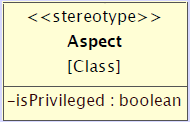
\includegraphics[width=100px]{img/p21_meta_class.png}
	\caption{Exemplo de estereótipo estendendo uma meta-classe em um diagrama de Perfil UML.}\label{fig:p21_meta_class}
\end{figure}

O Perfil UML completo proposto por Evermann pode ser visualizado na figura \ref{fig:p21_aspectj_profile}. Como todas as construções são definidas em
linguagem de meta-modelo, pode-se realizar a geração de código em AspectJ. É de responsabilidade do desenvolvedor elaborar uma modelagem que esteja de acordo 
com as construções da linguagem alvo para geração do código. 

\begin{landscape}
\begin{figure*}
	\centering
	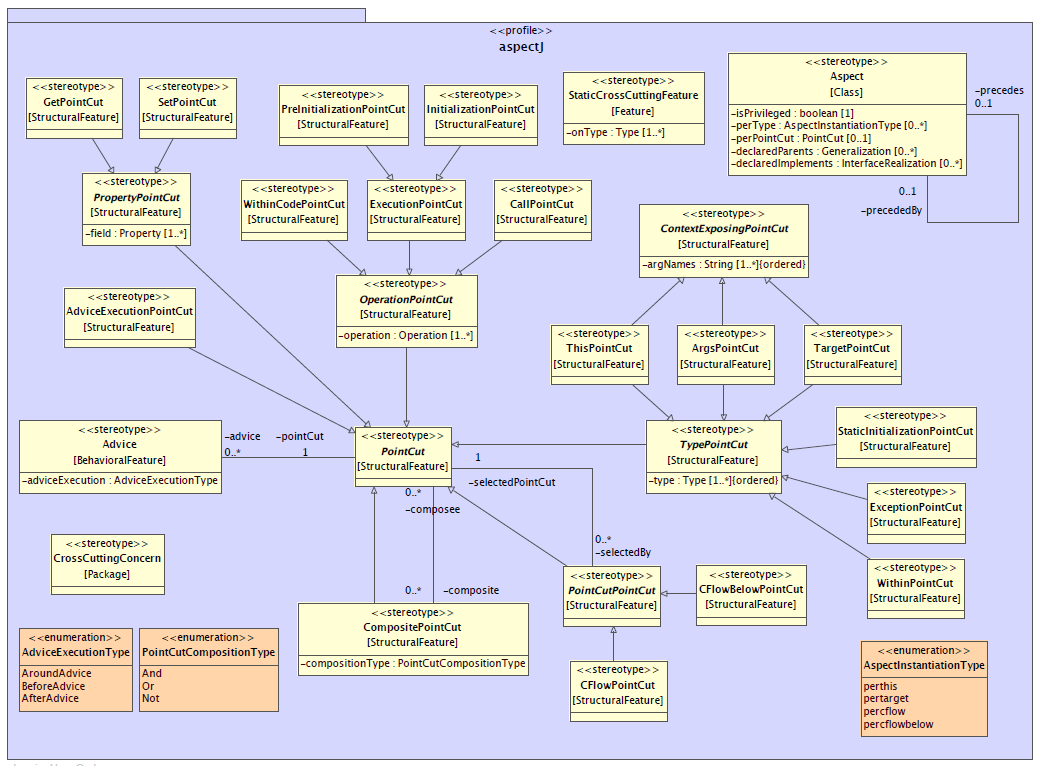
\includegraphics[scale=0.6]{img/p21_aspectj_profile.png}
	\caption{Perfil UML para modelagem de aspectos \cite{Evermann:2007:MSP:1229375.1229379}}\label{fig:p21_aspectj_profile}
\end{figure*}
\end{landscape}

Para exemplificar o uso deste Perfil UML em uma modelagem, Evermann implementou o padrão de projeto Observador \cite{Gamma:1995:DPE:186897} em um
sistema para desenho de interface gráfica. O diagrama de classes do interesse núcleo pode ser visualizado na figura \ref{fig:p21_base_model}. 

\begin{landscape}
\begin{figure*}
	\centering
	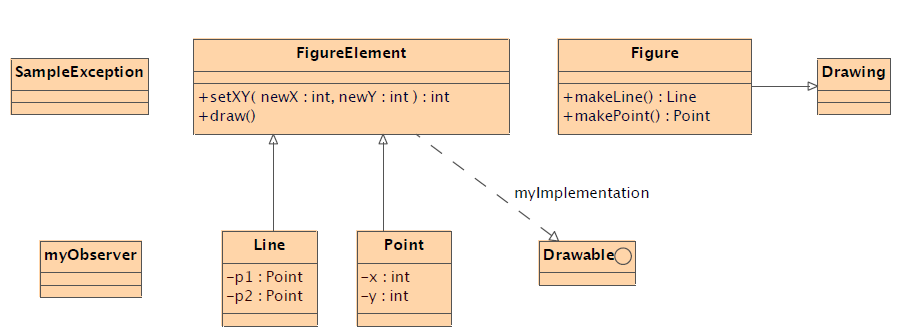
\includegraphics[scale=0.8]{img/p21_base_model.png}
	\caption{Interesse núcleo para desenho de interface gráfica}\label{fig:p21_base_model}
\end{figure*}
\end{landscape}

\begin{landscape}
\begin{figure*}
	\centering
	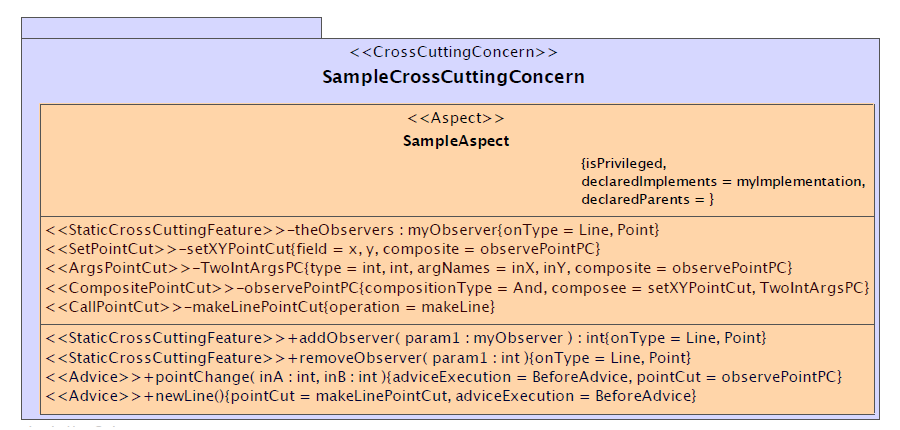
\includegraphics[scale=0.8]{img/p21_extension_model.png}
	\caption{Interesse entrecortante para implementação do padrão de projeto Observador}\label{fig:p21_extension_model}
\end{figure*}
\end{landscape}

O interesse entrecortante é o padrão de projeto Observador e a sua modelagem  pode ser visualizada na figura \ref{fig:p21_extension_model}. 
O modelo do interesse entrecortante contém um aspecto que especifica quatro pontos de corte, três introduções e dois avisos. O ponto de corte
\textit{setXYPointCut} captura modificações nos atributos x e y da classe \textit{Point}. O ponto de corte  \textit{twoIntArgsPC} captura chamadas e
execuções com dois argumentos do tipo inteiro. O ponto de corte \textit{observePointPC} compõe os dois pontos de cortes anteriores com o operador \textit{And},
capturando modificações nos atributos x e y da classe \textit{Point} com dois argumentos do tipo inteiro. Finalmente, define-se o ponto de corte 
\textit{makeLinePointCut} que captura chamadas ao método \textit{makeLine()}. As introduções adicionadas são os métodos \textit{addObserver()} e
\textit{removeObserver()} e o atributo \textit{theObservers} nas classes \textit{Line} e \textit{Point}. Estes membros permitem adicionar, remover e
armazenar os observadores. Para introduzir os novos comportamentos, especifica-se o aviso \textit{pointChange} que é executado antes do ponto de
corte \textit{observePointPC} e o aviso \textit{newLine} que é executado antes do ponto de corte \textit{makeLinePointCut}. A composição do interesse
entrecortante no interesse núcleo pode ser visualizada na figura \ref{fig:p21_code}. A composição é realizada em nível de código.

\begin{figure}
	\centering
	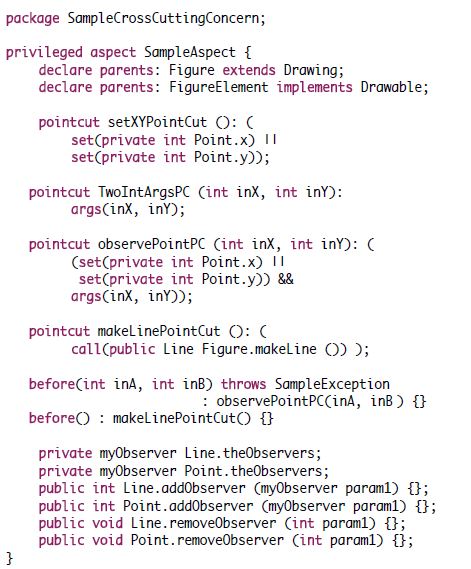
\includegraphics[width=300px]{img/p21_code.png}
	\caption{Composição do padrão observador no sistema de interface gráfica (em nível de código)}\label{fig:p21_code}
\end{figure}

A principal contribuição deste trabalho é a especificação do meta-modelo apenas em termos da UML, sem a necessidade de descrições textuais e de
ferramentas adicionais para interpretação ou geração de código a partir do modelo. Além disso, o meta-modelo pode ser utilizado como um perfil UML em
ferramentas que suportem a importação de perfis. Com a representação de elementos apenas em termos de meta-modelo, perde-se a possibilidade de
representar padrões para captura de pontos de junção: os \textit{wildcards}. A especificação por padrões é uma funcionalidade da programação por aspectos, pois simplifica a forma de capturar pontos de junção, sem a necessidade de explicitar cada elemento que
será capturado. Assim, é importante que a extensão à UML permita representar essas características de uma maneira simples e praticável, para que seja
possível expressar todas as características da POA na modelagem.

O trabalho de \cite{Evermann:2007:MSP:1229375.1229379} permite representar a estrutura de um programa orientado a aspectos através das meta-classes
\textit{CrossCutingConcern}, \textit{Aspect}, \textit{PointCut} e \textit{StaticCrossCutingFeatures}. É importante observar que apenas a parte
estrutural é especificada por esta proposta. Em relação às características comportamentais, como a meta-classe \textit{Advice} estende a meta-classe
\textit{BehavioralFeature}, é possível representá-las com colaborações e diagramas de máquinas de estados, mas o trabalho não demonstra como realizar
a modelagem de colaborações e nem permite a composição automatizada entre modelos que representam aspectos comportamentais do sistema. Assim,
conclui-se que o foco do trabalho é a representação da estrutura de um sistema orientado a aspectos. A parte comportamental deve ser implementada
manualmente no código gerado, que é uma limitação da abordagem, pois o desenvolvedor não pode especificar e visualizar o comportamento de aspectos nos
modelos que representam o sistema.

\section{Modelos de Aspectos Reusáveis (RAM) Proposto por Kienzle}

Uma modelagem por múltiplos pontos de vista é proposta por Kienzle \cite{Kienzle:2009:AMM:1509239.1509252} \cite{Kienzle2010}. Propõe-se RAM
(\textit{Reusable Aspects Models}), uma abordagem para especificar aspectos com dois diagramas comportamentais (diagrama de máquina de estados e de
sequência) e um diagrama estrutural (diagrama de classes). O objetivo deste trabalho é a melhora da escalabilidade de um sistema, mantendo a consistência entre as diferentes visões de um interesse
entrecortante. RAM define modelos base para representar interesses núcleo e de aspectos para representar interesses entrecortantes.

Duas ferramentas são utilizadas para a composição dos modelos. \textit{Kompose} \cite{kompose:07} é utilizado para composição da parte estrutural
(diagramas de classe). Para composição, os elementos do modelo devem ser instâncias da mesma classe do meta-modelo. A composição é realizada
comparando a assinatura de tipo dos elementos. Cada elemento do modelo deve possuir uma assinatura de tipo que o representa unicamente na modelagem.
Dois elementos que tiverem a mesma assinatura podem ser compostos. A composição de diagramas de sequência e de estado é realizada utilizando uma outra
ferramenta denominada GeKo \cite{geko:08}. Com essa ferramenta, para inserção de um novo comportamento em um modelo núcleo deve-se definir um modelo 
entrecortante (aspecto). Esse modelo de aspecto é composto por um diagrama refinando o ponto de corte e outro diagrama refinando o aviso. A composição
acontece em duas fases: primeiramente são detectados os elementos do modelo núcleo que são impactados pelo ponto de corte do modelo do aspecto. Com os 
elementos capturados executa-se um mecanismo de composição que gera o modelo composto com o comportamento (aviso)
do modelo do aspecto inserido no modelo núcleo (antes, durante ou depois). Essas duas ferramentas permitem representar aspectos e a composição entre
um modelo núcleo e um modelo de aspecto.

Um interesse em RAM é modelado através de um pacote UML. Este pacote contém três visões: estrutural, de estado e de mensagens e é denominado modelo de
um aspecto, podendo ser reusado em diferentes aplicações. A visão estrutural é composta por diagrama de classes. Nesta visão, as classes não precisam
ser completamente especificadas, pois só precisam expressar o que é relevante para o interesse em questão. A visão de estado descreve o protocolo de
uso de uma classe. Para classes completas, utiliza-se o diagrama de máquina de estados da UML. Classes incompletas são modeladas com um diagrama de
máquina de estados para aspectos, composto por uma parte representando o ponto de corte e outra representando o aviso. O ponto de corte determina
quais estados devem existir para o aviso ser executado. A visão de troca de mensagens utiliza o diagrama de sequência, onde cada método público das
classes modeladas deve ser representando. Aqui também pode-se especificar o comportamento de aspectos através de dois diagramas de sequência:
um para o ponto de corte e outro para o aviso. O ponto de corte determina a sequência de mensagens que deve ocorrer pra ativar o aviso. O aviso
descreve a sequência de mensagens que substituem o ponto de corte em uma execução. Nas três visões, alguns elementos podem estar incompletos, o que
significa que eles não são especificados no modelo de aspecto e deverão ser especificados por algum outro modelo na composição de modelos. Esses
elementos são denominados \textbf{parâmetros de instanciação mandatória}, identificados pelo prefixo | e modelados como parâmetros de
\textit{template} UML.

RAM permite estabelecer dependências entre aspectos, com o objetivo de possibilitar o reuso de modelos. Se um aspecto A depende de um aspecto B, A
deve instanciar todos os parâmetros de instanciação mandatória de B através de \textbf{diretivas de instancialização}. Por exemplo, para uma
classe incompleta em B, A deve especificar uma classe que possa completá-la com os métodos e atributos faltantes. Esta regra vale também para as visões de
estado e de mensagens. Além disso, A pode definir \textbf{diretivas de ligação} que mapeiam entidades incompletas de A em entidades completas de B.
Nesse caso, as entidades incompletas de A não podem ser parâmetros de instanciação mandatória. É importante observar que diretivas de ligação e
parâmetros de instanciação mandatória podem ser definidos com \textit{wildcards}, permitindo a captura de padrões.

A proposta de Kienzle também realiza a verificação de consistências entre as diferentes visões e modelos de aspectos. São realizadas verificações em
diferentes níveis:

\begin{itemize}
  \item \textbf{No modelo de aspecto}: Pode-se verificar se existe um diagrama de máquina de estados para cada classe na visão estrutural.
  \item \textbf{Entre modelos de aspectos}: Pode-se verificar que um aspecto A que depende de B deve inicializar todos os parâmetros de instanciação
  mandatórios de B.
  \item \textbf{No modelo final}: Pode-se comparar a sequência de mensagens na visão de mensagens com o diagrama de máquina de estados. As mensagens
  devem obedecer o protocolo do diagrama de máquina de estados.
\end{itemize}

Um estudo de caso foi realizado para avaliar a modelagem por múltiplos pontos de vista. No estudo adiciona-se a funcionalidade de garantia de
atomicidade em um modelo de transações. O modelo de transações bancárias (modelo núcleo) pode ser visualizado na figura \ref{fig:p87_base_model}. Para
garantir a atomicidade de transações utiliza-se o aspecto \textit{Recovering} que tem dependência com nove aspectos. Este aspecto pode ser visualizado 
na figura \ref{fig:p87_recovering_aspect.png}. Uma das dependências indiretas é o aspecto \textit{Checkpointable} (\textit{Recovering} depende de
\textit{Checkpointing} que depende de \textit{Checkpointable}). Este aspecto permite estabelecer pontos de verificação de um objeto, armazenando o seu estado e permitindo a restauração do mesmo. O aspecto \textit{Checkpointable} depende 
de um outro aspecto denominado \textit{Copyable} e ele deve instancializar os elementos incompletos de \textit{Copyable}. Um exemplo de
instancialização pode ser visualizado na visão de mensagens do aspecto \textit{Checkpointable}. A diretiva de instancialização \textit{clone.ICaller-ICheckpointable} 
indica que o objeto \textit{ICaller} da visão de mensagens do método \textit{clone} em \textit{Copyable} está sendo instancializado com o objeto
\textit{ICheckpointable} de \textit{Checkpointable}. O aspecto \textit{Recovering} também contém diretivas de instancialização para os elementos 
incompletos dos aspectos os quais depende.

\begin{landscape}
\begin{figure}
	\centering
	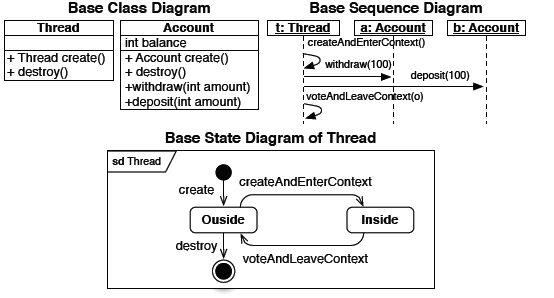
\includegraphics[scale=0.8]{img/p87_base_model.png}
	\caption{Modelo núcleo para transações}\label{fig:p87_base_model}
\end{figure}
\end{landscape}

Com o aspecto para garantia de atomicidade definido, deve-se realizar a composição com o modelo núcleo. O modelo final após a composição pode ser
visualizado nas figuras \ref{fig:p87_class_final_model} (visão estrutural), \ref{fig:p87_state_final_model} (visão de estados) e \ref{fig:p87_sequence_final_model} (visão de mensagens). 
Observa-se a presença de alguns elementos referentes ao aspecto \textit{Checkpointable} no modelo final como a classe \textit{Stack} e a inserção dos métodos \textit{establish(),
restore()} e \textit{discard()} na visão de mensagens. Na visão de troca de mensagens, as mensagens referentes ao aspecto \textit{Checkpointable}
também estão destacadas. Nesta visão, as mensagens de cada aspecto dependente estão destacadas. Assim, o modelo final contém uma parte de cada
aspecto, compostas com o modelo núcleo, resultando em um modelo que representa o comportamento desejado para garantia de atomicidade de transações.

\begin{landscape}
\begin{figure}
	\centering
	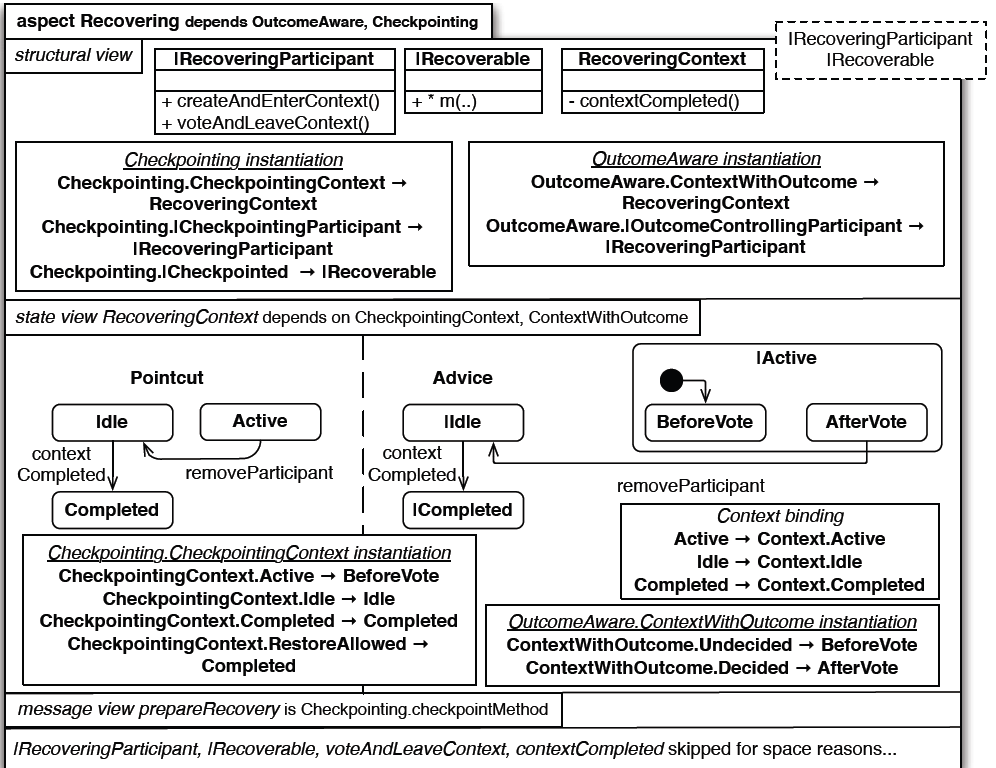
\includegraphics[scale=0.5]{img/p87_recovering_aspect.png}
	\caption{Aspecto para recuperação de dados (garantia de atomicidade)}\label{fig:p87_recovering_aspect.png}
\end{figure}
\end{landscape}

\begin{landscape}
\begin{figure}
	\centering
	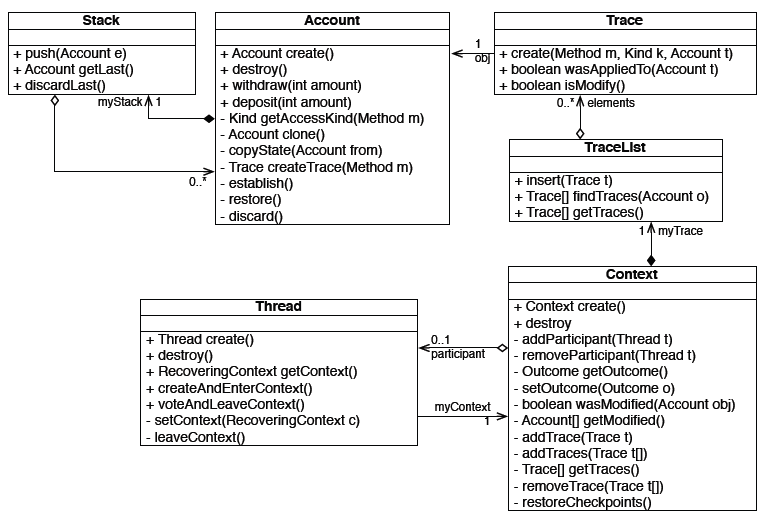
\includegraphics[width=500px]{img/p87_class_final_model.png}
	\caption{Visão estrutural do modelo final para garantia de atomicidade de transações}\label{fig:p87_class_final_model}
\end{figure}
\end{landscape}

\begin{landscape}
\begin{figure}
	\centering
	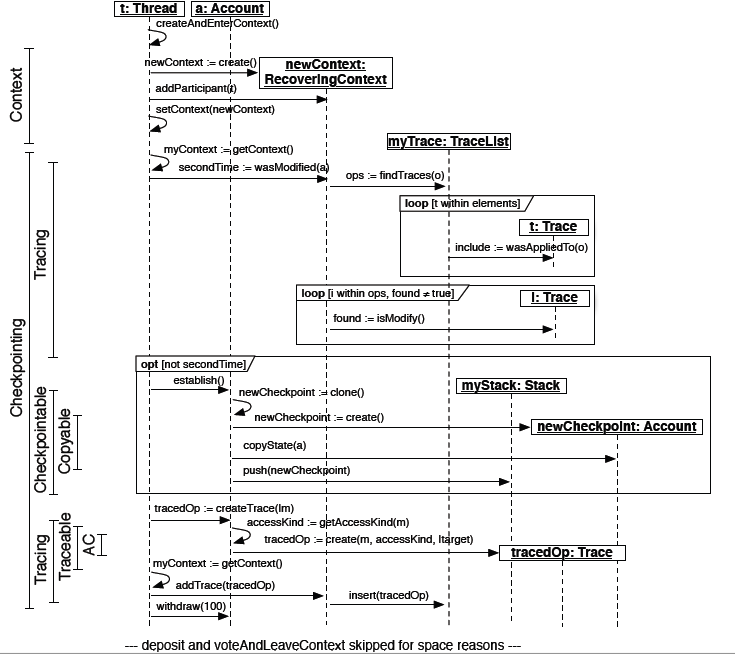
\includegraphics[scale=0.7]{img/p87_sequence_final_model.png}
	\caption{Visão de mensagens do modelo final para garantia de atomicidade de transações}\label{fig:p87_sequence_final_model}
\end{figure}
\end{landscape}

\begin{landscape}
\begin{figure}
	\centering
	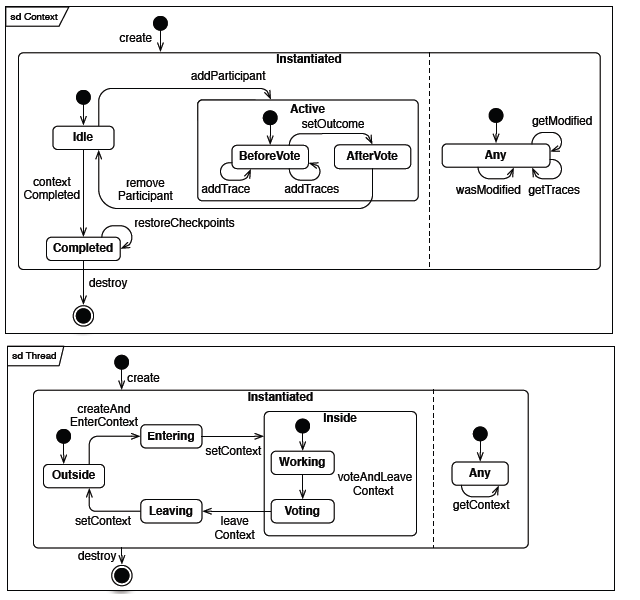
\includegraphics[scale=0.7]{img/p87_state_final_model.png}
	\caption{Visão de estados do modelo final para garantia de atomicidade de transações}\label{fig:p87_state_final_model}
\end{figure}
\end{landscape}

A abordagem RAM permite representar a estrutura de ums sistema através da visão estrutural e comportamental do sistema através das visões de estado
e de troca de mensagens. A maior contribuição deste trabalho é o foco na representação das caracaterísticas comportamentais de um sistema, utilizando
diagramas de máquinas de estado para representar o protocolo de um aspecto e diagramas de sequência para representar as possíveis interações entre
objetos. A especificação de pontos de corte com padrões (\textit{wildcards}) também é suportada pela ferramenta. Outra característica de RAM é a garantia de consistência entre as
diferentes visões e a orientação ao reuso de aspectos através da definição de dependências. 

Uma limitação da proposta é que nem todos os diagramas podem ser elaborados apenas estendendo a UML, pois a abordagem realiza modificações no
meta-modelo da UML, introduzindo novos conceitos que não estão presentes na versão padrão da OMG. Exemplos são as diretivas de instancialização e as diretivas de ligação. 
A complexidade do modelo composto também pode ser considerada uma limitação da abordagem, pois o modelo gerado é extenso, o que dificulta a
compreensão, já que existem muitas dependências indiretas entre aspectos e muitos elementos sintáticos na modelagem. Segundo \cite{seventwo:11},
quando uma pessoa entra em contato com novas informações, o limite de sua memória de trabalho é entre três ou quatro elementos de informação. A
modelagem proposta por Kienzle é difícil de ser compreendida, pois o modelo final (composto) contém muitos
elementos de informação. No exemplo de composição de aspectos, o modelo final contém elementos que vieram de nove diferentes aspectos. Além disso, contém elementos
que não são padrões na modelagem de sistemas com UML, como as diretivas de instancialização e de ligação. Para facilitar a compreensão do
comportamento de uma modelagem, este trabalho poderia disponibilizar um visualizador de aspectos, que permitisse habilitar e desabilitar
modelos de aspectos dinamicamente em um modelo núcleo, diferenciando os aspectos no modelo final.

\section{Modelagem de Aspectos com Atividades Proposto por Cui}

O trabalho de Cui, \cite{Cui:2009:MIA:1529282.1529377} modela o comportamento de um sistema com diagramas de atividades da segunda versão da UML. Os
interesses núcleo são modelados com a versão padrão da UML. No caso dos interesses entrecortantes, é proposta uma extensão ao diagrama de atividades com
estereótipos e valores rotulados. Um interesse entrecortante é representado por dois modelos: um para o ponto de corte e outro para o aviso.
Adiciona-se o estereótipo \textit{Pointcut} para indicar que um diagrama de atividades representa um \textbf{modelo de ponto de corte}. O estereótipo
\textit{Pointcut} tem um valor rotulado denominado \textit{advice} que aponta para o nome do modelo de aviso associado a este ponto de corte. Para
representar os pontos de execução de um programa que serão capturados adiciona-se o estereótipo \textit{Joinpoint}. Esta abordagem permite a seleção
de pontos de junção com o uso de \textit{wildcards}. Um elemento no modelo de ponto de corte estereotipado com \textit{Argument} define os argumentos
que serão passados para o modelo de aviso. O estereótipo \textit{Argument} tem um valor rotulado denominado \textit{parameter} que define o nome dos
parâmetros que serão preenchidos no modelo de aviso. O estereótipo \textit{Advice} é adicionado para especificar que um diagrama de atividades
representa um \textbf{modelo de aviso}. O valor rotulado \textit{type} está associado com este estereótipo indicando o tipo de aviso: antes ou depois.
O estereótipo \textit{Parameter} é adicionado para representar os parâmetros que são aceitos pelo modelo de aviso. Estes parâmetros são utilizados
para possibilitar o reuso de avisos, apenas modificando os parâmetros passados na inicialização. Finalmente, adicionam-se dois estereótipos
\textit{Entry} e \textit{Exit} para especificar o início e o fim de uma execução de um modelo de aviso.
 
\begin{figure}
	\centering
	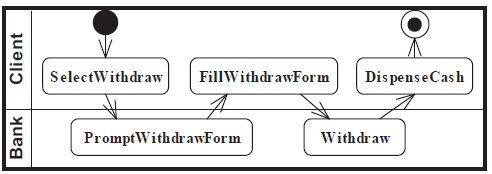
\includegraphics[width=300px]{img/withdraw_base.png}
	\caption{Modelo núcleo para realizar a transação de saque}\label{fig:withdraw_base}
\end{figure}

 A figura \ref{fig:withdraw_base} mostra o modelo núcleo de um caso de uso para realizar a transação bancária de saque. Este modelo é estendido
 utilizando a abordagem proposta por Cui, com a definição de dois pontos de corte e dois avisos. Os modelos do primeiro ponto de corte e do
 primeiro aviso podem ser visualizados na figura \ref{fig:withdraw_1}. O ponto de corte \textit{Pointcut1} seleciona os elementos no modelo núcleo
 aonde o aviso de autorização deve ser aplicado. O aviso \textit{Advice1} representa o comportamento de autorização. A figura \ref{fig:withdraw_2}
 mostra o ponto de corte \textit{Pointcut2} que pretende capturar os elementos no modelo núcleo aonde o aviso de envio de e-mail será
 aplicado. O aviso \textit{Advice2} representa o comportamento de enviar um e-mail. Observa-se uma diferença no comportamento dos dois avisos: a
 autorização é realizada antes (aviso do tipo \textit{before}) da execução dos pontos de junção selecionados pelo primeiro ponto de corte. No entanto,
 o envio de e-mail é realizado depois (aviso do tipo \textit{after}) dos pontos de junção selecionados pelo segundo ponto de corte, e, o envio de
 e-mail é realizado paralelamente ao comportamento dos pontos de junção. 

\begin{figure}
	\centering
	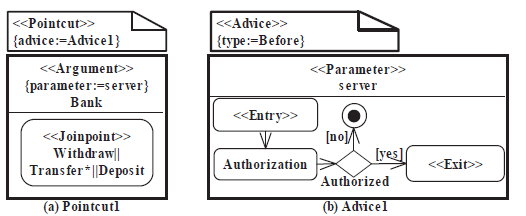
\includegraphics[width=300px]{img/withdraw_1.png}
	\caption{Ponto de corte e aviso para capturar pontos
	de junção que necessitam de autorização antes de
	serem executados}\label{fig:withdraw_1}
\end{figure}

Após a definição do modelo núcleo e dos modelos para os interesses entrecortantes, deve-se realizar a composição entre os modelos. Esta composição
consiste em três passos:

\begin{itemize}
  \item \textbf{Captura}: Encontrar os pontos de junção no modelo núcleo.
  \item \textbf{Inicialização}: Inicializar os modelos de aspectos com os parâmetros obtidos do modelo núcleo.
  \item \textbf{Composição}: Realizar a composição entre os modelos de aspectos e o modelo núcleo.
\end{itemize}

Após a composição, obtém-se o modelo final com os interesses entrecortantes introduzidos. O modelo final pode ser visualizado na figura
\ref{fig:withdraw_final}.

\begin{figure}[!t]
	\centering
	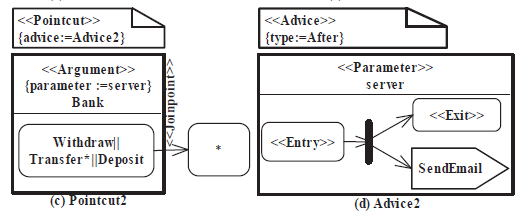
\includegraphics[width=300px]{img/withdraw_2.png}
	\caption{Ponto de corte para capturar pontos de junção onde é necessário
	enviar um e-mail após a execução dos mesmos}\label{fig:withdraw_2}
\end{figure}

A proposta de Cui é uma extensão à segunda versão da UML, estendendo apenas o diagrama de atividades com a adição de novos estereótipos e valores
rotulados para representar interesses entrecortantes. A extensão segue o padrão do meta-modelo definido pela OMG para a segunda versão da UML e 
pode ser utilizada em qualquer ferramenta que suporte a definição de perfis. É possível realizar a composição entre modelos de interesses núcleo e
modelos de interesses entrecortantes e a mesma é realizada em nível de modelo.

\begin{figure}
	\centering
	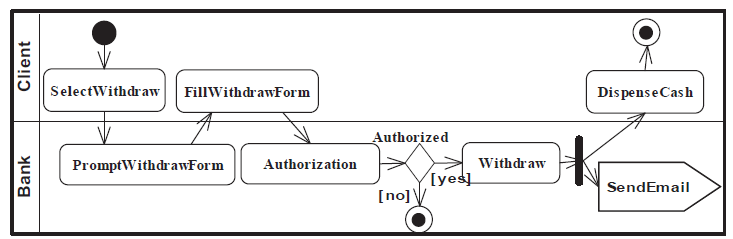
\includegraphics[width=275px]{img/withdraw_final.png}
	\caption{Modelo composto para transação bancária de
	saque com autorização e envio de e-mail}\label{fig:withdraw_final}
\end{figure}

Em relação a POA, a abordagem não permite representar as principais características do paradigma. Não é possível adicionar introduções a classes e
interfaces nos modelos de interesses núcleo. Também não é possível representar todos os tipos de ponto de junção e nem adicionar avisos do tipo \textit{around}, que permite
substituir a execução de um ponto de junção ou modificar o comportamento de execução do mesmo. Em relação as visões representadas pela modelagem, a
parte estrutural não pode ser representada apenas com diagrama de atividades e a abordagem não utiliza nenhum diagrama estrutural para representar o
sistema. Assim, esta proposta representa apenas a parte comportamental de um sistema orientado a aspectos. A principal contribuição desta proposta é
uma extensão leve e simples aos diagramas de atividades da UML para representação do comportamento de aspectos em alto nível de abstração.

\section{Modelagem de Aspectos com Casos de Uso Proposto por Jacobson}

O trabalho de Jacobson \cite{Jacobson:2004:ASD:1062430} utiliza casos de uso para representação de interesses entrecortantes. São identificados dois
tipos de caso de uso:

\begin{itemize}
  \item \textit{Peer Use Cases}: São casos de uso que não tem relacionamentos com outros casos de uso, mas sua implementação impacta mais de uma
  classe. São os interesses núcleo de um sistema.
  \item \textit{Extension Use Cases}: São casos de uso que estendem o comportamento de um caso de uso base. Tem relacionamentos com outros casos de
  uso e sua implementação pode impactar mais de uma classe. São os interesses entrecortantes de um sistema.
\end{itemize}

Propõe-se uma construção denominada \textbf{fatia de caso de uso} (\textit{use-case slice}) que deve modelar apenas as especificidades de um 
caso de uso. Para tal adiciona-se o estereótipo \textit{use-case slice} ao meta-modelo da UML. Uma fatia de caso de uso contém: definições de novas
classes necessárias para realizar o caso de uso, extensões a classes existentes (apenas a extensão será representada na fatia do caso de uso) e
colaborações para representar a realização do caso de uso. O gráfico da figura \ref{fig:jacobson_slices} mostra o impacto dos casos de uso nas classes
de um sistema de gerenciamento de hotel. Observa-se que os casos de uso \textit{Reserve Room}, \textit{Check In Customer} e \textit{Check Out
Customer} modificam a mesma classe \textit{Room}. Cada fatia de caso de uso define uma parte desta classe. A classe completa é obtida realizando a
composição das fatias de caso de uso. A classe \textit{StaffScreen} é modificada pelos casos de uso \textit{CheckOutCustomer} e
\textit{CheckInCustomer}. Já a classe \textit{Reservation} é modificada pelos casos de uso \textit{ReserveRoom} e \textit{CheckInCustomer}. As outras
classes são modificadas por apenas um caso de uso.

\begin{figure}
	\centering
	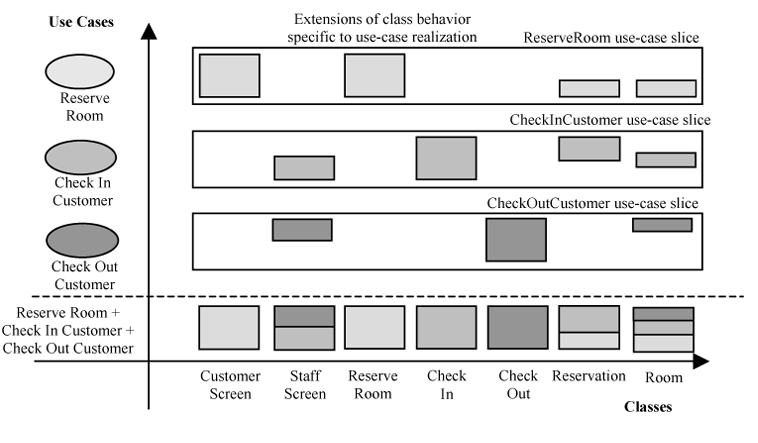
\includegraphics[width=350px]{img/jacobson_slices.png}
	\caption{Fatias de casos de uso em um sistema de
	gerenciamento de hotel}\label{fig:jacobson_slices}
\end{figure}

A figura \ref{fig:jacobson_reserve_room_slice} mostra a fatia do caso de uso \textit{Reserve Room}. As classes pertencentes a este interesse
estão dentro de um pacote estereotipado como \textit{use case slice}. Observa-se nesta figura o aspecto \textit{ReserveRoom} marcado com o estereótipo
\textit{aspect}. Dentro deste aspecto definem-se extensões à três classes do modelo: \textit{CustomerMainForm}, \textit{Reservation} e \textit{Room}.
A representação de extensões à classes é equivalente às introduções da linguagem AspectJ. Esta fatia de caso de uso define também
duas novas classes: \textit{ReserveRoomForm} e \textit{ReserveRoomHandler}. Este caso de uso é do tipo \textit{peer} (\textit{Peer Use Case}), pois
ele não estende nenhum caso de uso, apenas define novas classes e introduz métodos em classes já existentes.

\begin{figure}
	\centering
	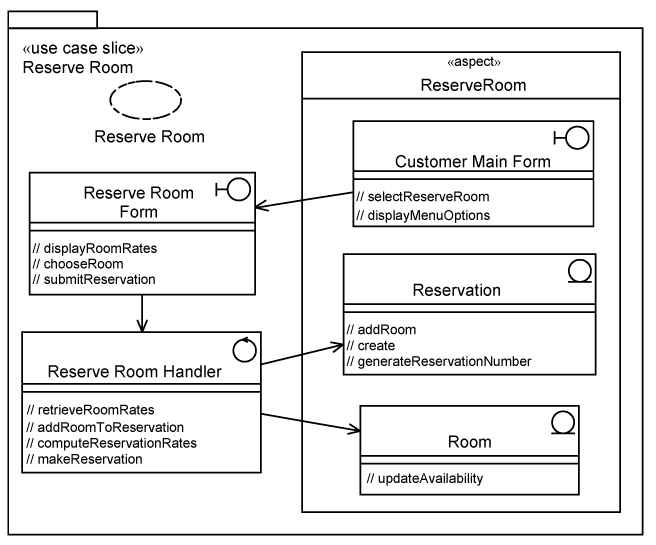
\includegraphics[width=300px]{img/jacobson_reserve_room_slice.png}
	\caption{Fatia de caso de uso para o
	caso de uso \textit{Reserve Room}}\label{fig:jacobson_reserve_room_slice}
\end{figure}

Os casos de uso de extensão (\textit{Extension Use Cases}) estendem o comportamento de um caso de uso base. A figura
\ref{fig:jacobson_use_case_extension} mostra o caso de uso \textit{Handle Waiting List} que estende o caso de uso \textit{Reserve Room}. Um caso de
uso base define um conjunto de \textbf{pontos de extensão} representando os pontos que podem ser estendidos por outros casos de uso. Um caso de uso de
extensão define \textbf{pontos de corte de extensão} para representar quais pontos de extensão do caso de uso base serão estendidos. 

\begin{figure}
	\centering
	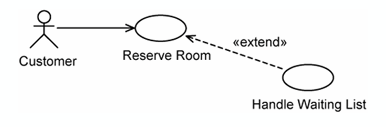
\includegraphics[width=300px]{img/jacobson_use_case_extension.png}
	\caption{Caso de uso de extensão
	\textit{Handle Waiting List}}\label{fig:jacobson_use_case_extension}
\end{figure}

A fatia de caso de uso da figura \ref{fig:jacobson_handle_waiting_list_slice} mostra a modelagem do caso de uso de extensão \textit{Handle Waiting
List}, que adiciona o cliente em uma lista de espera se não for possível reservar um quarto. Para tal, o caso de uso de extensão define o ponto de
corte \textit{updatingRoomAvailability} para capturar as chamadas ao método \textit{UpdateAvailability()} da classe \textit{Room}. Dentro do aspecto
define-se uma extensão à classe \textit{ReserveRoomHandler}, adicionando o método \textit{makeReservation()}. Este método será executado depois
do ponto de corte \textit{updatingRoomAvailability} quando forem lançadas as exceções \textit{NoRoomAvailable} ou \textit{QueueForRooms}. Além disso,
são introduzidos dois novos métodos à classe \textit{Reservation} relativos a reserva de quartos. Esta fatia de caso de uso cria duas novas classes:
\textit{WaitingListHandler} e \textit{WaitingList}.

\begin{figure}
	\centering
	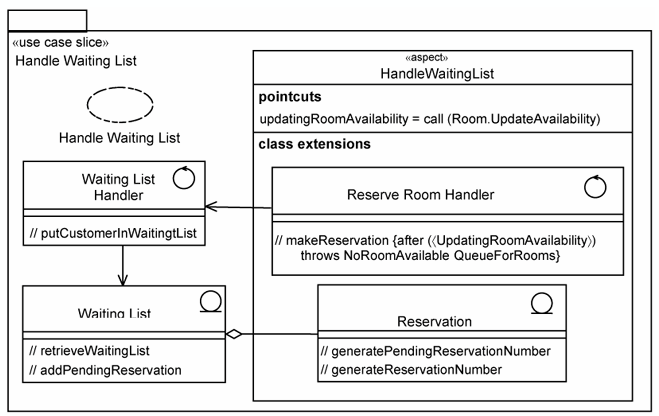
\includegraphics[width=300px]{img/jacobson_handle_waiting_list_slice.png}
	\caption{Fatia do caso de uso de extensão \textit{Handle Waiting List}}\label{fig:jacobson_handle_waiting_list_slice}
\end{figure}

A proposta de Jacobson propõe a definição de \textbf{modelos de caso de uso} para agrupar as fatias de caso de uso em
diferentes níveis de abstração. Define-se o estereótipo \textit{use-case module} no meta-modelo. São propostos quatro níveis de modelo: caso de uso,
análise, projeto e implementação. A fatia de caso de uso será refinada de acordo com o nível de abstração. Esta proposta consegue obter o rastreamento
completo do requisito para o código que o implementa, passando pelos modelos de caso de uso, análise e projeto, como pode ser visualizado 
na figura \ref{fig:jacobson_use_case_modules}. 

\begin{figure}
	\centering
	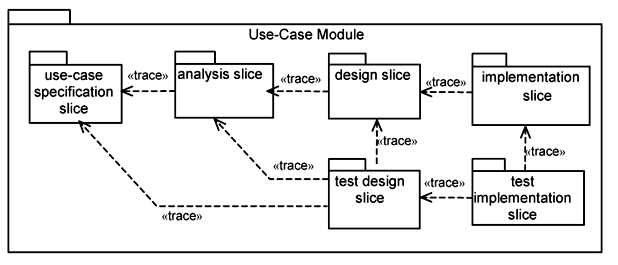
\includegraphics[width=350px]{img/jacobson_use_case_modules.png}
	\caption{Rastreamento completo de um requisito por todos modelos}\label{fig:jacobson_use_case_modules}
\end{figure}

Após a definição das fatias de caso de uso em diferentes níveis de abstração, deve-se compor os modelos de caso de uso para se obter um sistema
completo com o comportamento de cada caso de uso inserido nas respectivas classes. A figura \ref{fig:jacobson_use_case_merge} mostra a composição de
três modelos de casos de uso (cada modelo representado como um pacote UML) para gerar uma construção válida do sistema. Para tal utiliza-se o
estereótipo \textit{merge} que representa dependência entre pacotes.

\begin{figure}
	\centering
	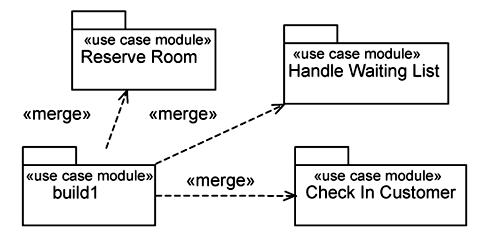
\includegraphics[width=350px]{img/jacobson_use_case_merge.png}
	\caption{Composição entre modelos de caso de uso}\label{fig:jacobson_use_case_merge}
\end{figure}

A proposta de Jacobson permite representar \textit{wildcards} na definição de pontos de corte dentro de uma fatia de caso de uso. Uma contribuição deste trabalho é a possibilidade de obter o rastreamento completo de um requisito até o código que o implementa. Segundo \cite{wimmer:2011:SUA:1978802.1978807}, 
o mapeamento de requisitos entre as diferentes fases do desenvolvimento é importante na modelagem de sistemas orientados a aspectos, como para
sistemas desenvolvidos em outros paradigmas como programação orientada a objetos. Em relação as diferentes visões representadas por uma modelagem, os
modelos propostos por este trabalho permitem representar a estrutura de um sistema com fatias de caso de uso e diagramas de classes. O comportamento
do sistema é representada através de colaborações que são associadas às fatias de caso de uso. Colaborações podem ser utilizadas para descrever a
dinâmica de casos de uso e avisos. Outro ponto a ser destacado é a representatividade do exemplo utilizado para realizar uma modelagem com
a proposta. O sistema de gerenciamento de hotel é complexo e contém interesses entrecortantes de diversos tipos, possibilitando a representação de boa
parte das características inerentes a programas orientados a aspectos.

Em relação as limitações do trabalho de Jacobson, a principal delas é a forma de extensão à UML, com a definição de um meta-modelo, que não pode ser utilizado 
em qualquer ferramenta CASE. Este meta-modelo tem construções específicas, como fatias de caso de uso, que não são suportadas por ferramentas CASE que
obedecem os padrões da segunda versão da UML. Destaca-se também a falta de ferramental para composição dos modelos, o que é importante para que seja
possível visualizar o impacto dos interesses entrecortantes nos interesses núcleo do sistema. Não é possível realizar a composição de pontos de corte entre modelos e visualizar a conexão entre os pontos de corte e os avisos nos modelos. Assim, a abordagem proposta por
Jacobson não permite visualizar completamente o efeito dos aspectos nos modelos núcleo do sistema. A geração automática de modelos também diminui o
tempo necessário para realização de uma modelagem, diminuindo o tempo de entrega ao cliente. Nesta proposta, a composição entre interesses núcleos e
interesses entrecortantes deve ser realizada manualmente, com o uso de diagramas de sequência, o que demanda um esforço adicional de modelagem.

\section{Motorola WEAVR Proposto por Cottenier}

Uma das unidades de negócio mais importantes da Motorola também está focada no desenvolvimento de soluções para modelagem de programas orientados a
aspectos. O trabalho de Cottenier \cite{Cottenier06themotorola} \cite{Cottenier:2007:SAC:1229375.1229377} foi desenvolvido na unidade de negócios empresariais e de redes da
Motorola. O projeto é denominado de \textbf{Motorola WEAVR} e é focado na especificação de sistemas de telecomunicações, que são sistemas reativos
discretos e orientados a eventos. Um sistema reativo é um sistema que recebe uma entrada e deve emitir uma reação a este estímulo. Já um sistema discreto é um sistema cuja
interação ocorre em eventos discretos no tempo. A motivação para este trabalho foi a percepção de que existem muitas mudanças nos requisitos de 
sistemas de telecomunicação ao longo do desenvolvimento. A modularização de interesses facilita a manutenabilidade e a inserção de novos requisitos ao
longo do ciclo de vida desse tipo de sistema. 

Motorola WEAVR permite a composição de aspectos que são modelados \textbf{com diagramas de máquina de estados focadas em transições}. Este tipo de
máquina de estado é uma extensão à máquina de estados da UML focada em estados, com o objetivo de prover um maior nível de detalhe na dinâmica das
transições. Segundo Bjorkander \cite{Bjorkander:2000:GPU:619058.621607}, o diagrama de máquina de estados focado em estados da UML não dá a atenção
que as transições merecem. Estas máquinas de estado ignoram as ações que ocorrem durante uma transição. A linguagem Specification and Description Language
(SDL) \sigla{SDL}{Specification and Description Language} \cite{sdl:00} foca nas ações que acontecem durante uma transição. Esta linguagem é
amplamente utilizada para especificar sistemas orientados a eventos na área de telecomunicações. Assim, a extensão proposta foca nas ações que ocorrem
durante uma transição e estende o diagrama de máquina de estados da UML com novas construções que permitem representar as ações de uma transição. O
diagrama de máquina de estados focado em transições permite diminuir o nível de abstração de uma modelagem, aproximando-o ao código
e permitindo a geração de código em uma linguagem alvo. A modelagem de ações que ocorrem durante transições já está disponível na especificação
do diagrama de máquina de estados da segunda versão da UML através deu um perfil UML \cite{uml:05}.

Esta abordagem também utiliza diagramas de estrutura composta da segunda versã da UML para especificar as interfaces do sistema e os componentes em
termo de sinais necessários e realizados. Este tipo de diagrama raramente é modificado durante o ciclo de vida de um sistema, por isso não são
utilizados na modelagem de programas orientados a aspectos. O diagrama da figura \ref{fig:weavr_composite_structure} mostra um diagrama de estrutura
composta para representar a estrutura de um servidor de recursos. Um servidor de recursos é composto por um despachante \textit{Dispatcher} e por um
ou mais tratadores de requisições \textit{RequestHandler}. O despachante tem a responsabilidade de passar requisições externas para um dos tratadores
de requisições. Um tratador de requisições é responsável por controlar o acesso a recursos, permitindo o acesso apenas se todos os recursos
necessários estiverem disponíveis. Esse tipo de controle pode ser implementado com o protocolo \textit{Two Phase Commit} \sigla{2PC}{Two Phase
Commit}.

\begin{figure}
	\centering
	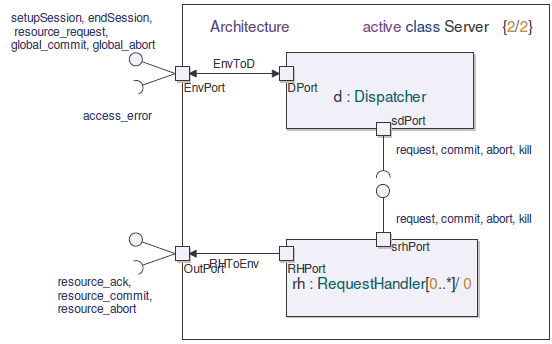
\includegraphics[width=350px]{img/weavr_composite_structure.png}
	\caption{Diagrama de Estrutura Composta
	representando um servidor de recursos}\label{fig:weavr_composite_structure}
\end{figure}

Após modelar a estrutura do sistema, deve-se modelar o comportamento de cada um dos componentes do servidor. Para tal, utilizam-se os diagramas de
máquina de estado focados em transições. Estes diagramas são utilizados para representar o comportamento de um componente em detalhes (sem
ambiguidades). Um diagrama deste tipo destaca o fluxo de controle e as ações executadas durante as transições entre os diferentes estados. A figura
\ref{fig:weavr_state_machine_base} representa a modelagem do comportamento de um tratador de requisições.

\begin{figure}
	\centering
	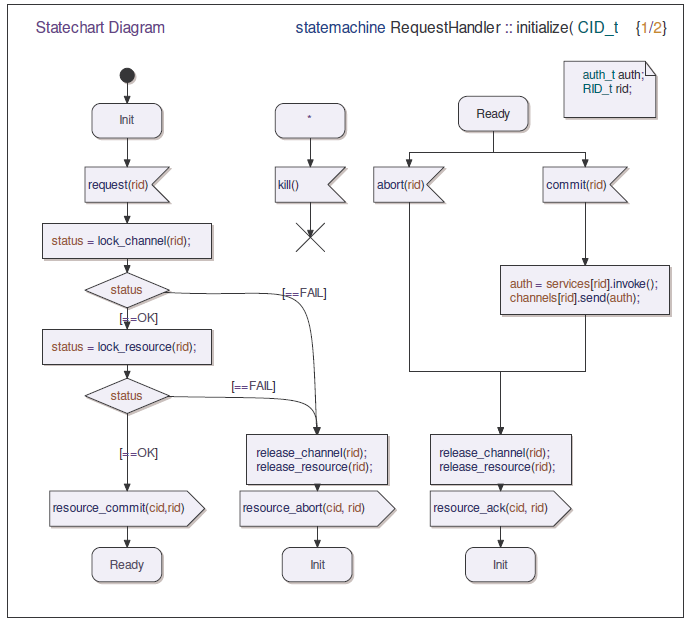
\includegraphics[width=350px]{img/weavr_state_machine_base.png}
	\caption{Diagrama de máquina de estados focado em transições
	para um tratador de requisições}\label{fig:weavr_state_machine_base}
\end{figure}

Observando o primeiro diagrama de máquina de estados, verifica-se a presença de um conjunto de ações entre os estados \textit{Init} e \textit{Ready}. 
A primeira ação \textit{request(rid)} indica o recebimento de um sinal para iniciar uma requisição. A segunda ação dentro de um retângulo tenta
adquirir o canal e armazena o resultado na variável \textit{status}. Após estas ações está presente um nodo decisão para verificar a variável
\textit{status}. Se o resultado for um \textit{OK}, significa que o canal foi adquirido com sucesso e executa-se uma nova ação para adquirir o recurso
desejado, armazenando o resultado na variável \textit{status}. Se o valor da variável \textit{status} no nodo decisão for \textit{OK}, executa-se a
ação \textit{resource\_commit(cid,rid)} que indica o envio de um sinal. Este sinal indica que o recurso foi adquirido. Finalmente, atinge-se o estado
\textit{Ready}. Se em algum momento a variável \textit{status} retornar uma falha, o canal e o recurso serão liberados, abortando a acquisição do
recurso. Todas estas ações ocorrem durante o disparo de uma transição. 

No ambiente distribuído da Motorola existem vários sistemas que utilizam o protocolo 2PC no tratamento de requisições. Cada sistema implementa uma
variação deste protocolo. A implementação do protocolo apenas com POO é possível, mas gera um código emarranhado e de difícil manutenção, pois o
código do protocolo fica misturado com o código da aplicação. A POA permite implementar de maneira modular o protocolo 2PC. Esta foi uma das
motivações para criação da ferramenta \textbf{Motorola WEAVR}. 

Esta ferramenta define um perfil UML para modelagem de aspectos. A extensão proposta por Cottenier pode ser reutilizada em outras
ferramentas de modelagem. O perfil adiciona o estereótipo \textit{Aspect} que estende o elemento \textit{Class} do meta-modelo da UML. Um aspecto pode 
conter conectores e pontos de corte. Um conector é o equivalente a um aviso na terminologia de aspectos. O estereótipo
\textit{Connector} foi criado para representar um conector. Para representar pontos de corte utiliza-se o estereótipo \textit{Pointcut}. Estes
estereótipos estendem o elemento do meta-modelo \textit{Operation}. Conectores são associados a pontos de corte através do relacionamento de
dependência \textit{Binds}. A ordem de precedência de conectores é definida pelo relacionamento de dependência \textit{Follows}. O estereótipo
\textit{Crosscuts} define o escopo de aplicação de um aspecto. Se nenhum escopo for definido, indica que o aspecto é aplicado a todo o sistema.

A figura \ref{fig:weavr_timeout} mostra a implementação de um aspecto de controle de tempo (\textit{timeout}) para o protocolo 2PC. A motivação para
implementação deste aspecto é que o tratador de requisições da figura \ref{fig:weavr_state_machine_base} tem um problema: se uma instância entrar no
estado \textit{Ready}, mas não receber nenhum sinal do tipo \textit{Commit} ou \textit{Abort}, ela nunca terminará e não poderá receber
novas requisições. Para solucionar este problema, adiciona-se um tempo máximo para que esta instância receba um sinal. Ao final deste tempo, a
instância será destruída. Este comportamento é introduzido através do aspecto \textit{2PCTimeoutAspect} que pode ser visualizado na figura
\ref{fig:weavr_timeout}. 

\begin{figure}
	\centering
	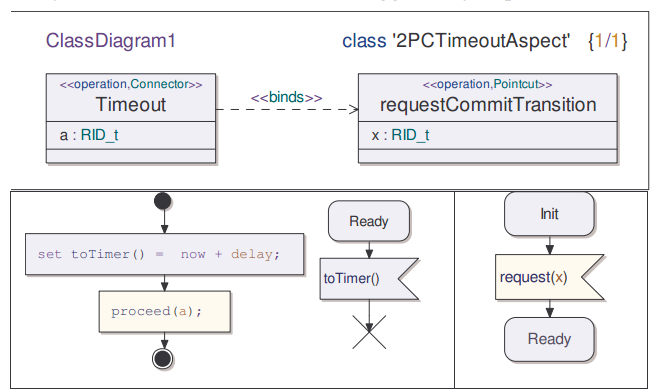
\includegraphics[width=325px]{img/weavr_timeout.png}
	\caption{Aspecto para controle de tempo ao protocolo 2PC}\label{fig:weavr_timeout}
\end{figure}

Um dos elemenos definidos neste aspecto é o ponto de corte \textit{requestCommitTransition}. A ferramenta WEAVR permite definir pontos de 
corte com o uso do diagrama de máquina de estados. Existem duas categorias de pontos de junção que que foram identificados nos diagramas de máquinas
de estado:

\begin{itemize}
  \item \textbf{Pontos de junção de ação}: Englobam as chamadas de operações, ações temporais e chamadas de construtores. 
  \item \textbf{Pontos de junção de transição}: Compreendem o conjunto de caminhos de execução dentro de uma máquina de estados.
\end{itemize}

O ponto de corte \textit{requestCommitTransition} captura pontos de junção de transição, pois captura execuções ao método \textit{request(x)} enquanto
uma instância estiver entre os estados \textit{Init} e \textit{Ready}, capturando um conjunto de caminhos de execução. Quando o ponto de corte for
disparado, executa-se o comportamento descrito no conector \textit{Timeout}. A ferramenta WEAVR representa a dinâmica de conectores através de
diagrama de máquina de estados. Este conector é refinado em duas máquinas de estado. A primeira máquina de estado representa a reinicialização do
contador de tempo antes das transições capturadas pelo ponto de corte. A segunda representa a destruição da instância ao atingir o tempo máximo sem
receber nenhum sinal.

Para visualizar o impacto de aspectos em um modelo núcleo, a ferramenta WEAVR disponibiliza um \textbf{visualizador do efeito de aspectos}. O
visualizador é uma importante contribuição deste trabalho, pois permite visualizar em quais pontos do modelo núcleo serão inseridos novos
comportamentos. Por exemplo, ao aplicar o aspecto \textit{2PCTimeoutAspect} (figura \ref{fig:weavr_timeout}) no tratador de requisições \textit{RequestHandler} 
(figura \ref{fig:weavr_state_machine_base}), o visualizador de aspectos gera a máquina de estados que pode ser visualizada na figura
\ref{fig:weavr_composed}. Esta máquina de estado mostra os locais da máquina de estado que são impactados pelo aspecto de controle de tempo. 
Os pontos de junção de ação são marcados com a cor roxo, enquanto os pontos de junção de transição são marcados com uma marca horizontal verde ao
longo das transições. O usuário pode clicar em um determinado ponto de junção para visualizar a máquina de estado do conector (aviso) que será executada 
naquele ponto. Observa-se na máquina de estados 15.a que a transição capturada é a transição que ocorre após o a variável \textit{status} retornar OK
até o estado \textit{Ready} (dois marcadores horizontais verdes). O conector que será disparado pode ser visualizado na máquina de estados 15.b e 
uma representação da transição capturada pode ser visualizada na máquina de estados 15.c.

\begin{figure}
	\centering
	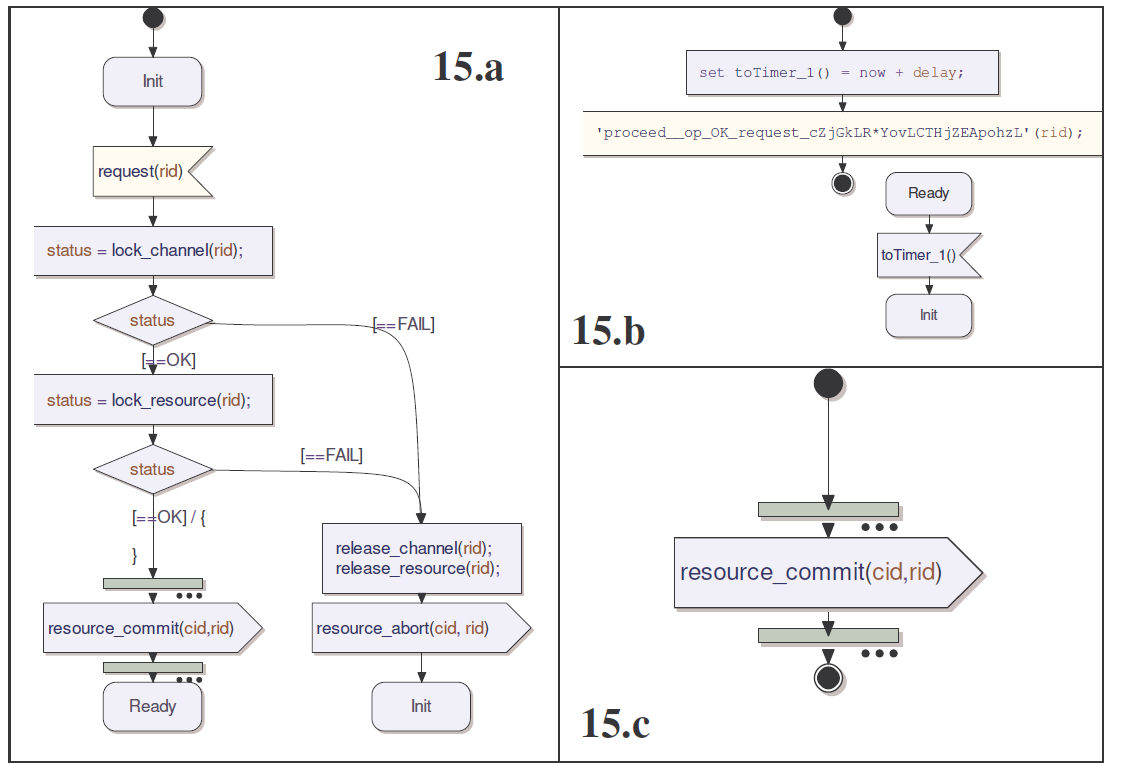
\includegraphics[width=350px]{img/weavr_composed.png}
	\caption{Visualização da composição do aspecto
	para controle de tempo no tratador de requisições.}\label{fig:weavr_composed}
\end{figure}

Motorola WEAVR também disponibiliza uma ferramenta para executar modelos de aspectos. Ao encontrar um conector, a ferramenta executa a máquina de
estado referente ao mesmo e retorna o controle a máquina de estado base. A possibilidade de executar um modelo de aspectos facilita a compreensão do
fluxo de execução de um programa orientado a aspectos. O trabalho de Cottenier estende a segunda versão da UML através de um perfil UML para
representar aspectos com diagramas de classes e diagramas de máquina de estados. Esta extensão pode ser importada em diferentes ferramentas CASE. 
Diagramas de classes permitem representar a parte estrutural de um sistema. Os diagramas de máquinas de estado são responsáveis por representar
o comportamento do sistema. Motorola WEAVR permite representar a maior parte das características de programas orientados a aspectos, como
\textit{wildcards}, pontos de corte, avisos, introduções e dependência entre aspectos. A ferramenta também disponibiliza ferramental para visualização, composição e execução de modelos de aspectos. Este ferramental é uma das principais contribuições do trabalho, pois automatiza parte do processo de modelagem e
permite gerar código em um linguagem alvo.

Uma limitação desta proposta, em relação a linguagem, é que apenas avisos do tipo durante (\textit{around}) são suportados. Outra desvantagem é o baixo nível 
de abstração dos modelos. Isto acontece, pois um dos focos do trabalho é a execução do sistema em nível de modelo, deixando os modelos  próximos do
nível de código. Os diagramas de máquinas de estado desta proposta contém trechos de código e código referente a POA, como chamadas ao método \textit{proceed()}. 
O baixo nível de abstração dificulta a compreensão dos modelos, pois o desenvolvedor precisa compreender chamadas próximas do nível de código. A
utilização de diagramas como os diagramas de caso de uso e de sequência permitiriam representar um sistema em um maior nível de abstração, facilitando a compreensão 
e manutenção do mesmo. 

\section{Modelagem de Aspectos com Diagramas de Sequência Proposto por Klein}

O trabalho de Klein \cite{Klein:2007:WMA:1805812.1805819} \cite{Klein:2006:SWS:1119655.1119662} propõe uma extensão aos diagramas de sequência da UML para permitir a modelagem
de sistemas orientados a aspectos. Esta extensão é realizada no meta-modelo da UML, estendendo o mesmo com a adição de novas classes, restrições e
relacionamentos. Separam-se os diagramas de sequência em dois tipos:

\begin{itemize}
  \item \textbf{bSD}: Diagrama de sequência básico que descreve um número finito de interações entre um conjunto de objetos. É equivalente ao diagrama
  de sequência padrão da UML.
  \item \textbf{cSD}: Diagrama de sequência composto que permite compor diagramas de sequência básicos através de operadores como nodos decisão
  e iterações. Este tipo de diagrama permire representar comportamentos infinitos e é semelhante ao diagrama de visão geral de interação.
\end{itemize}

O meta-modelo para diagramas de sequência pode ser visualizado na figura \ref{fig:klein_meta_model}. Observa-se a presença de duas classes que
derivam da super classe \textbf{SD}(\textit{SequenceDiagram}): \textbf{bSD}(\textit{BasicSequenceDiagram}) e
\textbf{cSD}(\textit{ComposedSequenceDiagram}). Um diagrama de sequência composto contém um conjunto de nodos e um conjunto de transições que estão
associadas a diagramas de sequência básicos.

\begin{figure}
	\centering
	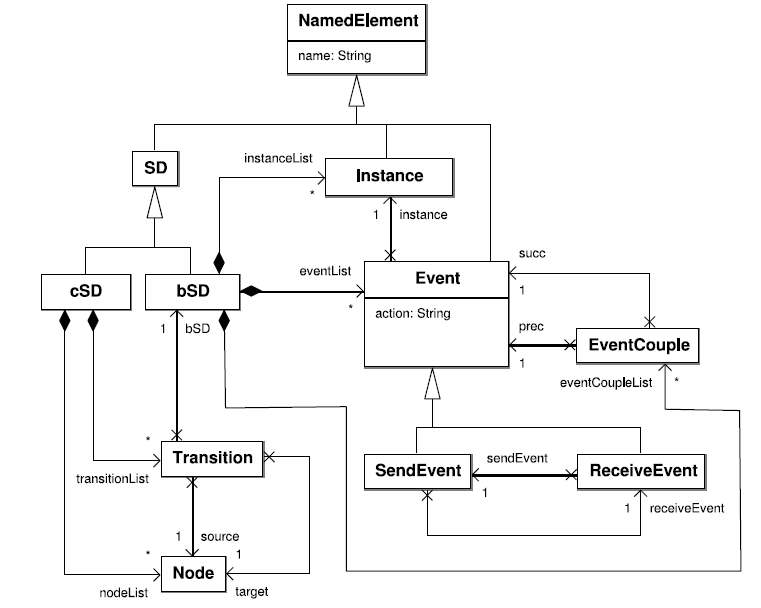
\includegraphics[width=350px]{img/klein_meta_model.png}
	\caption{Meta-modelo de extensão aos diagramas de
	sequência da UML}\label{fig:klein_meta_model}
\end{figure}

No lado esquerdo da figura \ref{fig:klein_sequence_diagrams} estão dispostos quatro bSD's: \textit{Propose}, \textit{Accept}, \textit{Retry} e
\textit{Rejected}. Estes bSD's representam etapas na interação com um servidor para realizar a autenticação de um usuário(\textit{log in}). O cSD
central e o cSD a direita são equivalentes e compõem os quatro bSD's a esquerda. Ambos cSD's especificam a autenticação de usuário(\textit{log in}). O
cSD central utiliza nodos decisão e o cSD a direita utiliza fragmentos do tipo \textit{alt} para representar diferentes caminhos de execução.

\begin{figure}
	\centering
	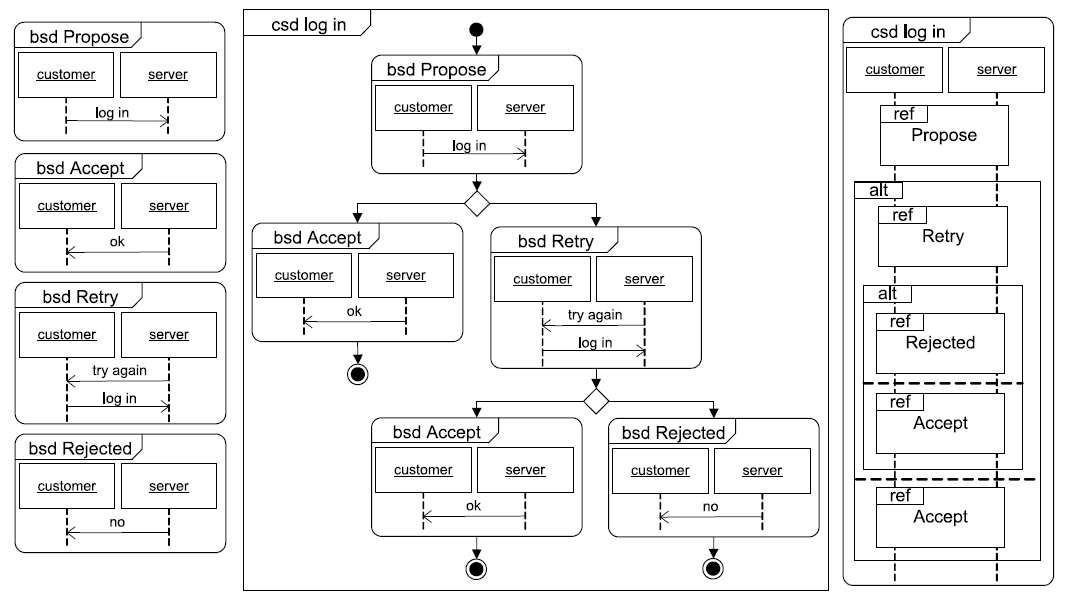
\includegraphics[width=350px]{img/klein_sequence_diagrams.png}
	\caption{Exemplos de diagramas de sequência
	estendidos: bSD's e cSD's}\label{fig:klein_sequence_diagrams}
\end{figure}

Para modelagem de aspectos deve-se definir um \textbf{aspecto comportamental} que é composto por dois bSD's: um para representar o ponto de corte e
outro para representar o novo comportamento (aviso). Um ponto de corte é representado como uma sequência de mensagens entre um conjunto de objetos. A
ferramenta não suporta a utilização de \textit{wildcards} na definição de pontos de corte, uma funcionalidade da POA, que permite a captura
de múltiplos pontos de junção em uma única declaração. Um aviso também é representado com bSD's e pode ser executado antes, durante ou depois dos
pontos de junção capturados por um ponto de corte. A figura \ref{fig:klein_aspects} mostra três aspectos comportamentais: registro de mensagens,
segurança e atualização de interface gráfica. O aspecto de segurança(\textit{Aspect Security}) define um ponto de corte que captura a troca das
mensagens \textit{log in} e \textit{try again} entre os objetos \textit{customer} e \textit{server}. O aviso que implementa o comportamento do aspecto
de segurança adiciona a mensagem \textit{save bad attempt} entre as mensagens \textit{log in} e \textit{try again}. Uma limitação nesta abordagem é
que o diagrama de sequência dos avisos é redundante, pois repete as mensagens capturadas no ponto de corte. No exemplo do aspecto de segurança, as
mensagens \textit{log in} e \textit{try again} são repetidas no aviso. Assim, se o ponto de corte for modificado, o aviso também deve ser modificado,
gerando um re-trabalho desnecessário. Na linguagem AspectJ, a modificação de um ponto de corte não gera modificações aos avisos associados aquele
ponto de corte.

\begin{figure}
	\centering
	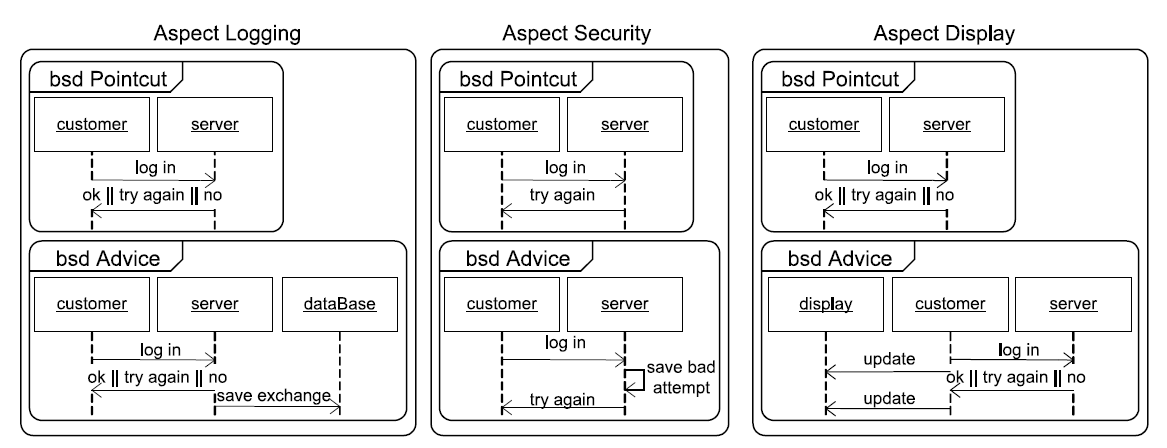
\includegraphics[width=350px]{img/klein_aspects.png}
	\caption{Exemplos de aspectos comportamentais}\label{fig:klein_aspects}
\end{figure}

Após definir os aspectos, deve-se realizar a composição dos aspectos em um modelo núcleo. O foco deste proposta é a composição de múltiplos aspectos
em um mesmo ponto de junção. Na composição de aspectos, o primeiro aspecto que for composto pode modificar a sequência de mensagens entre objetos no
modelo núcleo, fazendo com que o próximo aspecto não detecte o ponto de junção no qual o novo comportamento deveria ser inserido. Considerando a
composição entre o diagrama de sequência (cSD) \textit{log in} da figura \ref{fig:klein_sequence_diagrams} como modelo núcleo e os aspectos para
registro de mensagens, segurança e atualização de interface. Se o aspecto de segurança for o primeiro a ser composto, ele mudará a sequência de
mensagens entre os objetos \textit{customer} e \textit{server}, adicionando a mensagem \textit{save bad attempt} entre as mensagens \textit{log in} e
\textit{try again}. Se não existir um tratamento no algoritmo de detecção de pontos de junção,  os aspectos de registro de mensagens e atualização de
interface não capturarão os pontos de junção definidos por seus pontos de corte e a composição não será realizada corretamente. Assim, o algoritmo de
detecção de pontos de junção deve ser capaz de capturar pontos de junção, mesmo que existam mensagens introduzidas por outros aspectos durante a
composição de aspectos. A proposta de Klein resolve este problema detectando mensagens inseridas por outros aspectos durante a composição
de aspectos e permitindo a composição de múltiplos aspectos em um mesmo ponto de junção. A composição entre os aspectos e o modelo núcleo pode ser
visualizada na figura \ref{fig:klein_composition}.

\begin{figure}
	\centering
	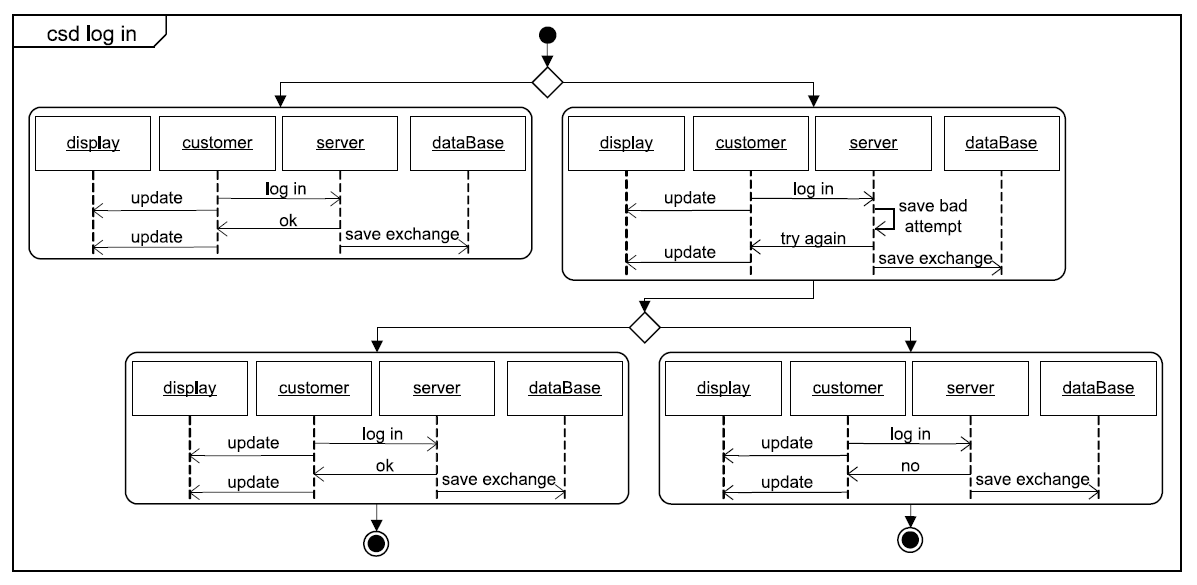
\includegraphics[width=350px]{img/klein_composition.png}
	\caption{Composição entre aspectos de registro de mensagens, segurança e 
	atualização de interface gráfica com modelo
	base para autenticação de usuário}\label{fig:klein_composition}
\end{figure}

Uma das limitações da proposta de Klein é a não representação da estrutura do sistema. A abordagem de Klein utiliza apenas diagramas de sequência para
modelagem do comportamento do sistema. Em relação a POA, não é possível representar introduções de membros em classes, uma funcionalidade da
linguagem. Não é possível utilizar \textit{wildcards} na definição de pontos de corte, o que torna difícil a captura de múltiplos pontos de junção em um mesmo ponto de corte. Além disso, a especificação de avisos contém redundâncias, pois replicam-se as mensagens referentes ao ponto de corte
capturado. A principal contribuição do trabalho é a possibilidade de realizar a composição de múltiplos aspectos em um mesmo ponto de junção, mantendo
as mensagens disparadas em cada aviso e identificando corretamente os pontos de junção, mesmo com mensagens introduzidas após a introdução de um
aviso. Em relação a forma de extensão à UML, as modificações da proposta não podem ser usadas diretamente em qualquer ferramenta CASE. Os modelos
gerados por esta proposta devem ser convertidos para o meta-modelo padrão da UML (através de transformações). A conversão de modelos não é tratada
neste trabalho, dificultando ainda mais o reuso da proposta em diferentes ferramentas CASE.

\section{Theme/UML Proposto por Clarke}

A proposta de Clarke \cite{clarke:04} permite realizar a análise e projeto de sistemas orientados a aspectos, desde a eliciação de requisitos,
passando pela modelagem e automatizando parte do processo com a composição automatizada de modelos núcleo com modelos de interesses entrecortantes
(aspectos). Na proposta elaborada por Clarke cada funcionalidade do sistema é considerada um tema (\textit{theme}). Os temas são identificados na fase
de levantamento de requisitos pela ferramenta Theme/Doc, que guia a obtenção de requisitos de sistemas orientados a aspectos. Para modelagem
estrutural utilizam-se os diagramas de pacote e de classes. Um pacote que representa um tema está associado ao estereótipo \textit{theme}, 
que representa um interesse do sistema. Diagramas de sequência são utilizados para modelagem comportamental. A modelagem de interesses
núcleo é realizada dentro dos padrões da UML, apenas marcando o pacote que define o tema com o estereótipo \textit{theme}. No entanto, a modelagem dos
interesses entrecortantes utiliza um mecanismo estendido de \textit{templates} da UML, que permite definir elementos não instancializados em um tema. 
Estes parâmetros serão instancializados posteriormente indicando quais elementos do modelo núcleo serão estendidos pelos interesses
entrecortantes. 

\begin{figure}
	\centering
	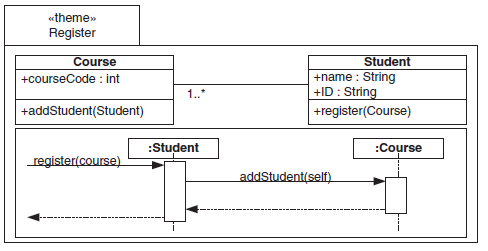
\includegraphics[scale=0.8]{img/theme_1.png}
	\caption{Modelo núcleo: registro de estudante em curso}\label{fig:theme_1}
\end{figure}

A figura \ref{fig:theme_1} apresenta um interesse núcleo para matrícula de um estudante em um curso. Observa-se a presença do estereótipo
\textit{theme} associado ao pacote que contém um diagrama de classes e um diagrama de sequência. A figura \ref{fig:theme_2} representa um interesse
entrecortante para registro de atividades do sistema, como o cadastro de um estudante em um determinado curso. Este tema contém um \textit{template}
UML com dois parâmetros. O primeiro parâmetro é o objeto do modelo núcleo que está sendo registrado e o segundo representa o método que está sendo
executado no modelo núcleo. Para realizar a composição de interesses, o desenvolvedor deve instancializar estes parâmetros com elementos do modelo
núcleo.

\begin{figure}
	\centering
	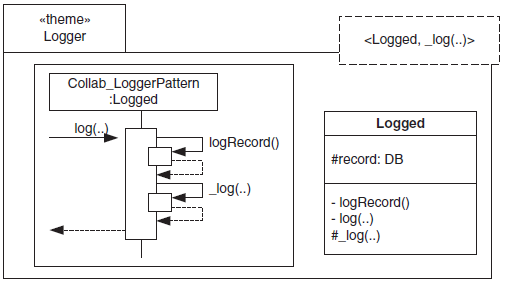
\includegraphics[scale=0.8]{img/theme_2.png}
	\caption{Modelo entrecortante: registro de atividades do sistema}\label{fig:theme_2}
\end{figure}

A figura \ref{fig:theme_3} apresenta uma configuração para composição de temas. Esta configuração define que objetos do tipo \textit{Person},
\textit{Student} e \textit{Professor} são objetos que podem ser alvo do registro de atividades. Além disso, define que os métodos que terão a
atividade registrada são: \textit{Student.register()}, \textit{Person.unregister()} e \textit{Professor.giveMark()}. Em relação a composição de
modelos, um plug-in para o ambiente de desenvolvimento Eclipse \cite{Eclipse} permite realizar a composição de modelos. O algoritmo de composição
recebe a modelagem em formato XMI como entrada e, baseado no meta-modelo proposto por Theme/UML, produz um modelo final independente de plataforma com
os modelos núcleo compostos com os interesses entrecortantes \cite{Carton:2009:MT:1692821.1692829}. 

\begin{figure}
	\centering
	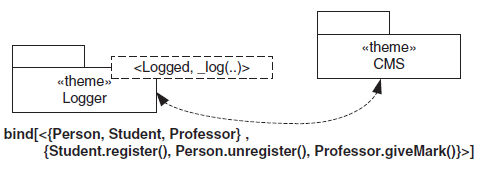
\includegraphics[scale=0.8]{img/theme_3.png}
	\caption{Configuração de composição entre interesses}\label{fig:theme_3}
\end{figure}

Uma importante contribuição da abordagem é a especificação de aspectos desde a eliciação de requisitos, passando pela modelagem até a composição de
modelos. As ferramentas Theme/DOC e Theme/UML também permitem realizar a rastreabilidade de interesses (temas), desde a fase de requisitos, modelagem 
até o projeto do sistema. Outra vantagem da abordagem de Clarke é a independência de plataforma em relação a linguagem para programação orientada a
aspectos. Theme/UML é projetado como uma abordagem independente de plataforma, com mapeamentos para AspectJ, AspectWerkz \cite{aspectwerkz} e Hyper/J
\cite{hyperj}.

Uma das limitações da proposta de Clarke é a forma de extensão à UML, pois a mesma estende o meta-modelo da UML. Esta forma de extensão limita o uso
da proposta de modelagem apenas em ferramentas próprias. O meta-modelo depende da versão 1.3 \textit{beta} da UML e não pode ser utilizado em
ferramentas CASE que suportem a importação de perfis. Com o objetivo de inserir a abordagem dentro dos padrões da segunda versão da UML, foi
desenvolvido um perfil UML baseado na versão 2.1 da linguagem \cite{Carton:2009:MT:1692821.1692829}. No entanto, este trabalho ainda depende do meta-modelo 
original, pois para realizar a composição deve-se transformar os estereótipos e valores rotulados para o meta-modelo original do Theme/UML. 

\section{Modelagem de Aspectos com Diretivas de Composição Proposto por France}

O trabalho de France \cite{france:06} \cite{FranceReddy} apresenta uma proposta para especificação e composição de modelos de aspecto com modelos
núcleo utilizando diretivas de composição. Os modelos de aspecto são descrições genéricas de interesses entrecortantes, que devem ser instancializadas antes de serem
compostas com um modelo núcleo. A instancialização ocorre através de \textit{templates} da UML, semelhante a abordagem proposta por Clarke
\cite{clarke:04}. Um modelo de aspecto pode ser instancializado mais de uma vez na mesma modelagem. A instancialização de um modelo de aspecto envolve 
atribuir valores a todos os parâmetros de um \textit{template} com valores do domínio da aplicação. Um diferencial da proposta de Clarke é que a
comparação entre elementos do modelo para realizar a composição de classes utiliza outras variáveis além do nome do elemento, como o tipo de retorno
de um método, o número e o tipo dos parâmetros, etc. A comparação e seleção de elementos impactados é baseada em uma assinatura ao invés de uma
simples comparação por nome.

Além da comparação de elementos pela sua assinatura, a proposta também disponibiliza as diretivas de composição, que permitem adicionar restrições e
verificações para a composição de modelos. Existem dois tipos de diretivas: de modelo e de elemento. As diretivas de modelo definem a ordem de
composição de modelos, isto é, a ordem que os aspectos são compostos. Já as diretivas de elemento determinam como um modelo de aspecto é composto em
um modelo núcleo. Um exemplo de diretiva de elemento é a adição de novos elementos em um modelo. Estes elementos são definidos em um modelo de aspecto
e devem ser inseridos no modelo composto. Já um exemplo de diretiva de modelo é a definição de precedência entre aspectos no momento da composição.
Esta diretiva especifica que um modelo de aspecto deve ser composto antes de outro modelo.

A figura \ref{fig:clarke_1} exemplifica o uso de diretivas de composição. O modelo núcleo a esquerda apresenta duas classes: \textit{Writer} e
\textit{FileStream}, que representam o comportamento de escrever linhas em um \textit{stream}. O modelo de aspecto a direita contém as mesmas duas
classes e adiciona uma outra classe para introduzir um \textit{buffer} de escrita (\textit{WriterBuffer}). Para realizar a composição entre estes dois
modelos deve-se adicionar algumas diretivas de composição. A primeira diretiva é a remoção da associação entre as classes \textit{Writer} e
\textit{FileStream}, pois agora a escrita passará por um \textit{buffer}. Além disso, remove-se a especificação Object Constraint Language (OCL)
\cite{ocl:12} do método \textit{writeLine()} no modelo primário. A remoção da especificação OCL e da associação entre classes podem ser visualizadas
na figura \ref{fig:clarke_2}, que mostra os modelos após a aplicação das diretivas de composição. Após a aplicação das diretivas, a composição de modelos pode ser realizada sem disparar conflitos entre
os elementos dos modelos.

As diretivas de composição são uma importante contribuição da proposta de France, pois elas permitem realizar a composição de diagramas de classe
prevendo e evitando a maior parte dos conflitos. O foco deste trabalho é a especificação e a composição da estrutura de aspectos. A parte
comportamental é tratada pelo trabalho de Reddy e Solberg \cite{ReddySolberg}, que estende a proposta e trata da especificação e composição 
de diagramas de sequência. No entanto, a composição de diagramas de sequência e a adição de um suporte ferramental para a composição dos mesmos ainda estão
sendo estudadas pelos autores. O trabalho de France e Reddy \cite{FranceReddy} estuda a implementação de uma ferramenta para composição dos modelos
estruturais automaticamente, sem esforço do desenvolvedor. Este suporte ferramental é desejável, pois automatiza parte do processo de modelagem,
diminuindo a quantidade de esforço manual necessária.

Uma das limitações da proposta de \cite{france:06} é a não representação de algumas características importantes da POA, como a captura de múltiplos
pontos de junção em uma única construção. A abordagem utiliza \textit{templates} da UML para instancializar os aspectos com elementos do domínio da
aplicação, mas não permite instancializar múltiplos elementos ao mesmo tempo. Outra limitação da abordagem é a falta de suporte ferramental para
realizar a composição de modelos comportamentais. Os modelos devem ser compostos manualmente pelo desenvolvedor. O suporte ferramental automatiza
parte do processo de modelagem, diminuindo o esforço do desenvolvedor e o tempo necessário para realizar a modelagem. A composição de modelos
comportamentais permite visualizar o efeito do comportamento dos modelos entrecortantes (aspectos) nos modelos núcleos, facilitando a compreensão de
um sistema orientado a aspectos.

\begin{landscape}
\begin{figure}
	\centering
	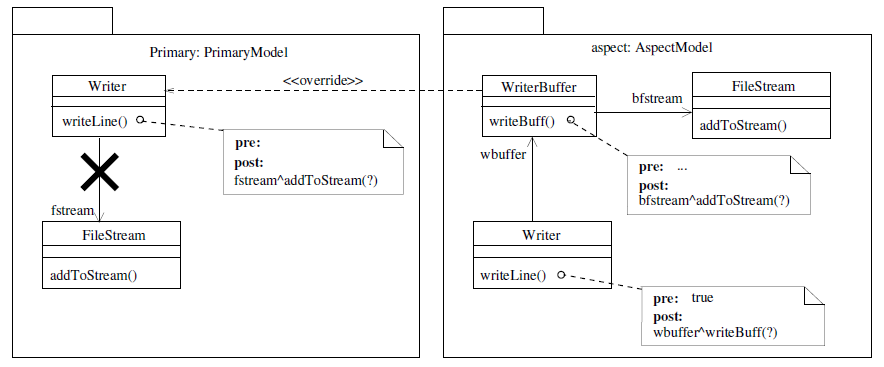
\includegraphics[scale=0.8]{img/clarke_1.png}
	\caption{Antes do uso de diretivas de composição para composição de aspectos}\label{fig:clarke_1}
\end{figure}
\end{landscape}

\begin{landscape}
\begin{figure}
	\centering
	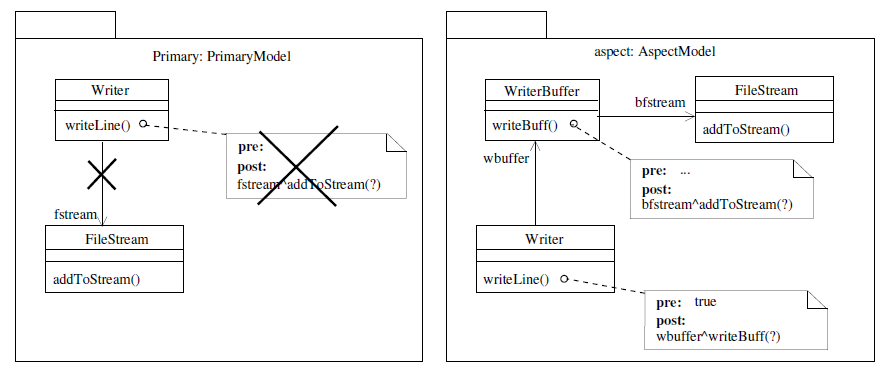
\includegraphics[scale=0.8]{img/clarke_2.png}
	\caption{Depois do uso de diretivas de composição para composição de aspectos}\label{fig:clarke_2}
\end{figure}
\end{landscape}

\section{Modelo de Projeto de Aspectos (AODM) Proposto por Stein}

A proposta de Stein (Aspect-Oriented Design Model (AODM)) \cite{stein:02} \cite{Stein02onrepresenting} \cite{stein:aosd-uml02} permite a especificação
de sistemas orientados a aspectos. A modelagem é baseada nas construções da linguagem AspectJ para implementação de aspectos utilizando Java. O
trabalho de Stein estende o meta-modelo da UML através de um perfil UML, adicionando estereótipos e valores rotulados. No entanto, algumas
construções estendem o meta-modelo da UML diretamente. Segundo os autores, propõe-se também uma composição em nível de modelo das construções
propostas pela linguagem AspectJ. A modelagem de aspectos é implementada utilizando diagrama de classes, colaborações da UML 1.x e casos de uso. Os
casos de uso são utilizados para definir a ordem de composição entre aspectos. A proposta permite a composição de aspectos e de introduções.

Para representar aspectos adiciona-se o estereótipo \textit{aspect} ao elemento do meta-modelo \textit{(Class)}. Um aspecto contém alguns parâmetros
de configuração, atributos, operações, pontos de corte e avisos. Pontos de corte são definidos com o estereótipo \textit{pointcut}, que 
estende \textit{(Operation)} e contém uma assinatura e uma declaração. A declaração define quais pontos de junção serão capturados nos modelos
núcleo. O estereótipo \textit{advice} também estende o elemento do meta-modelo \textit{Operation} e permite especificar avisos. 
Introduções são especificadas utilizando \textit{templates} da UML.  O estereótipo \textit{introduction} permite representar introduções de métodos,
classes, atributos e também de relacionamentos entre elementos. Antes de utilizar um \textit{template} que define uma introdução deve-se instancializar 
todos os parâmetros com argumentos do domínio de aplicação. 

O exemplo da figura \ref{fig:stein_1} apresenta um modelo de aspecto (AODM) segundo a proposta de Stein. O exemplo trata do padrão de projeto
observador/observado que permite que um observador escute mudanças em alguns objetos observados. A modelagem contém um aspecto abstrato que deve ser
estendido e um aspecto concreto que implementa o padrão de projeto. O aspecto abstrato (\textit{SubjectObserverProtocol}) contém um aviso do tipo
depois e um ponto de corte. O ponto de corte \textit{stateChanges} captura mudanças no estado de um objeto e deve ser especificado pelo aspecto
concreto. A semântica adicionada pelo aspecto abstrato é que os objetos observadores serão notificados quando ouver alguma mudança de estado nos
objetos observados. No entanto, o exemplo não apresenta como é modelado o comportamento do aviso. O aspecto concreto
(\textit{SubjectObserverProtocolImpl}) instancializa o padrão de projeto em uma aplicação, sobreescrevendo o ponto de corte \textit{stateChanges} para 
capturar cliques em um botão. Além disso, adiciona duas introduções às classes \textit{Button} e \textit{ColorLabel}. 

\begin{figure}
	\centering
	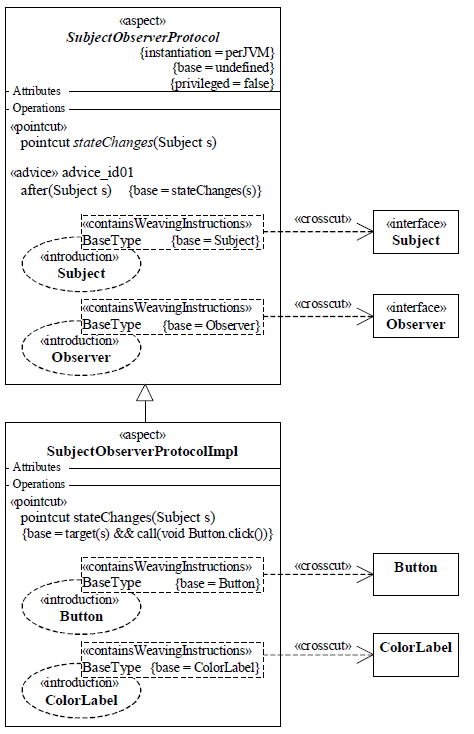
\includegraphics[scale=0.8]{img/stein_1.png}
	\caption{Um modelo de aspecto segundo a abordagem AODM}\label{fig:stein_1}
\end{figure}

Uma das limitações da proposta de Klein é a necessidade de estender o meta-modelo da UML. Embora a proposta utilize um perfil UML para adicionar estereótipos e valores rotulados, o meta-modelo da
UML é estendido. A extensão do meta-modelo não permite que a proposta seja utilizada em qualquer ferramenta CASE que suporte a importação de perfis.
Outra limitação do trabalho é a dependência com a primeira versão da UML, com o uso de diagramas de colaboração, que dependem de construções presentes
na primeira versão da linguagem. A falta de uma ferramenta para composição automática de modelos é outra limitação do trabalho, pois é necessário que o desenvolvedor
especifique todos os modelos manualmente, inclusive os modelos compostos.

\section{Comparação de Abordagens}

Existem algumas abordagens para modelagem de sistemas orientados a aspectos. Esta dissertação propõe uma comparação entre diferentes abordagens
considerando alguns critérios de comparação. Os critérios apresentados na seção \ref{sec:wimmer} são baseados no trabalho proposto por
Wimmer \cite{wimmer:2011:SUA:1978802.1978807}. A seção \ref{sec:ghilardi} apresenta os critérios propostos por este trabalho. Para permitir uma
melhor visualização das tabelas de comparação, as abordagens são abreviadas com as três primeiras letras do autor principal. 
Para cada critério, apresenta-se a tabela de comparação entre as abordagens e uma pequena discussão sobre os resultados de
cada tabela.

\subsection{Critérios Propostos por Wimmer}\label{sec:wimmer}

\subsubsection{Critérios de Linguagem}

\begin{itemize}
	\item \textbf{Linguagem para Modelagem (L.M)}: Diz respeito a linguagem utilizada para modelagem. Neste trabalho apenas abordagens que utilizam UML
	são estudadas. Logo, abordagens podem utilizar a versão 1.x ou a segunda versão da UML.
	\item \textbf{Mecanismo de Extensão (M.E)}: Abordagens para modelagem de sistemas orientados a aspectos podem estender a UML através de um perfil
	leve, que pode ser utilizado em ferramentas CASE que suportem a importação de perfis, ou adicionando novos elementos, restrições e relacionamentos ao
	meta-modelo da linguagem. A extensão através de perfis permite uma maior inter-operabilidade de abordagens para modelagem em diferentes ferramentas
	CASE \cite{Booch:2005:UML:1088874}.
	\item \textbf{Diagramas Estruturais (D.E)}: Quais diagramas estruturais são utilizados para descrever a estrutura de aspectos.
	\item \textbf{Diagramas Comportamentais (D.C)}: Quais diagramas comportamentais são utilizados para descrever o comportamento de aspectos.
\end{itemize}

A tabela \ref{tab:comparison_table_language} apresenta a comparação entre diferentes abordagens utilizando os critérios de linguagem.

\begin{landscape}
\begin{table*}[h]
	\centering
	\begin{tabular}{ | c | c | c | c | c | c | c | c | c | c | }
		\hline
		 & KLE & EVE & KIE & JAC & CUI & STE & COT & CLA & GHI \\
		\hline
		 L.M & 2.0 & 2.0 & 2.0 & 2.0 & 2.0 & 1.x & 2.0 & 2.0 (1.x) & 2.0 \\
		\hline
		 L.E & MM & P & MM & MM & P & MM & P & MM & P \\
		\hline
		 D.E & - & DC & DC & DC, DComp & - & DC & DC, DEC, DI & DP, DC & DP, DC\\
		\hline
		 D.C & DS & - & DS, DME & DS, DCom, DCU & DA & DCol & DME & DS & DS, DME \\
		\hline
	\end{tabular}
	
	\hspace{2em}

	\begin{tabular}{  p{16.6cm}  }
		Abreviações Autores: \\
	\end{tabular}
	
	\begin{tabular}{ | p{16.6cm} | }
		\hline
		KLE (Klein), EVE (Evermann), KIE (Kienzle), JAC (Jacobson), CUI (Cui), STE (Stein), COT (Cottenier), CLA (Clarke), GHI (Ghilardi) \\
		\hline
	\end{tabular}
	
	\begin{tabular}{  p{16.6cm}  }
		Legenda: \\
	\end{tabular}

	\begin{tabular}{ | p{16.6cm} | }
		\hline
		MM (Meta-Modelo), P (Perfil UML), DC (Diagrama de Classes), DComp (Diagrama de Componentes), DEC (Diagrama de Estrutura Composta), DI
		(Diagrama de Implantação), DP (Diagrama de Pacotes), DS (Diagrama de Sequência), DCol (Diagrama de Colaboração), DA (Diagrama de Atividades), 
		DME (Diagrama de Máquina de Estados), DCU (Diagrama de Casos de Uso) e DCom (Diagrama de Comunicação)\\
		\hline
	\end{tabular}
	\caption{Comparação entre abordagens: critérios de linguagem}
	\label{tab:comparison_table_language}
\end{table*} 
\end{landscape}

Observa-se que a maior parte das abordagens especificam aspectos com a segunda versão da UML. As abordagens limitadas a primeira versão da UML não contemplam todas 
as construções da linguagem e, não são suportadas por qualquer ferramenta CASE, diminuindo a expressividade da abordagem e a qualidade da mesma. Em
relação a forma de extensão, algumas abordagens estendem por um perfil UML, enquanto outras estendem diretamente o meta-modelo. A extensão por meta-modelo 
não permite utilizar a abordagem em outra ferramenta diferente da que foi implementada 
originalmente, diminuindo o potencial de reuso. Já um perfil UML pode ser importado em ferramentas CASE que suportem a importação de perfis,
possibilitando o reuso em ferramentas CASE comerciais. A maior parte das abordagens utiliza diagramas de classe para modelagem estrutural. Em relação
ao comportamento, a maior parte das abordagens modela com diagramas de sequência. Na especificação comportamental, alguns abordagens utilizam o
diagrama de máquina de estados, que permite representar em mais detalhes o comportamento de sistemas orientados a aspectos, como a modelagem de pontos
de corte.

\subsubsection{Critérios de Composição e Modelos}

\begin{itemize}
	\item \textbf{Composição Simétrica (C.S)}: Este critério analisa quais modelos de interesses podem ser compostos com outros modelos. Na modelagem de
	sistemas orientados a aspectos, em algumas abordagens, o modelo do interesse entrecortante (aspecto) é modelado diferentemente do modelo núcleo.
	Nesses casos, a composição é assimétrica, pois apenas modelos de interesses entrecortantes podem ser compostos em modelos núcleo. A composição
	simétrica acontece quando não há diferenciação entre modelos entrecortantes e modelos núcleo, podendo realizar a composição entre qualquer modelo.
	\item \textbf{Nível de Abstração (N.A)}: Distingue o nível de abstração dos elementos das abordagens. As abordagens podem representar construções de
	sistemas orientados a aspectos em alto ou baixo nível de abstração. É possível que uma abordagem represente conceitos nos dois níveis. Abordagens que
	representam conceitos em nível de código são classificadas como de baixo nível de abstração, enquanto abordagens que utilizam apenas modelos estão em
	alto nível de abstração.
	\item \textbf{Composição Estrutural (C.E)}: Avalia se a abordagem permite realizar a composição estrutural de modelos.
	\item \textbf{Composição Comportamental (C.C)}: Avalia se a abordagem permite realizar a composição do comportamento de modelos.
	\item \textbf{Ferramenta para Modelagem (F.M)}: Distingue abordagens que disponibilizam uma ferramenta para modelagem, de abordagens que não
	disponibilizam uma ferramenta que auxilie a modelagem. Abordagens que estendem a UML através de um perfil automaticamente disponibilizam este suporte, pois o perfil
	pode ser importado em outras ferramentas CASE.
	\item \textbf{Ferramenta para Composição (F.C)}: Algumas abordagens disponibilizam uma ferramenta para composição automática da estrutura e
	comportamento de modelos, possibilitando visualizar o comportamento de aspectos inserido no sistema, sem esforço do desenvolvedor. 
\end{itemize}

A tabela \ref{tab:comparison_table_models} apresenta a comparação entre diferentes abordagens utilizando os critérios de composição e modelos.

\begin{table*}[h]
	\centering
	\begin{tabular}{ | c | c | c | c | c | c | c | c | c | c | }
		\hline
		 & KLE & EVE & KIE & JAC & CUI & STE & COT & CLA & GHI \\
		\hline
		 C.S & sm & - & asm & asm & sm & - & sm & sm & sm \\
		\hline
		 N.A & alto & baixo & alto & alto & alto & baixo & baixo & alto & alto \\
		\hline
		 C.E & não & não & sim & não & não & não & sim & sim & sim \\
		\hline
		 C.C & sim & não & sim & não & sim & não & sim & sim & sim \\
		\hline
		 F.M & não & sim & sim & não & não & não & sim & sim & sim \\
		\hline
		 F.C & não & não & não & não & não & não & sim & não & sim  \\
		\hline
	\end{tabular}
	
	\hspace{2em}

	\begin{tabular}{  p{12cm}  }
		Abreviações Autores: \\
	\end{tabular}
	
	\begin{tabular}{ | p{12cm} | }
		\hline
		KLE (Klein), EVE (Evermann), KIE (Kienzle), JAC (Jacobson), CUI (Cui), STE (Stein), COT (Cottenier), CLA (Clarke), GHI (Ghilardi) \\
		\hline
	\end{tabular}

	\begin{tabular}{  p{12cm}  }
		Legenda: \\
	\end{tabular}

	\begin{tabular}{ | p{12cm} | }
		\hline
		sm (Modelos Simétricos), asm (Modelos Assimétricos) \\
		\hline
	\end{tabular}
	\caption{Comparação entre abordagens: critérios de composição e modelos}
	\label{tab:comparison_table_models}
\end{table*} 

Em relação à modelagem simétrica ou assimétrica, a maior parte das abordagens especifica os interesses entrecortantes com construções diferentes dos
interesses núcelo. A maior parte das abordagens representa aspectos em alto nível de abstração. A modelagem em alto nível de abstração facilita a
compreensão e manutenção do sistema. Boa parte das abordagens permite a modelagem de sistemas orientados a aspectos. Abordagens que estendem a
linguagem através de um perfil podem ser utilizadas em outras ferramentas CASE, possibilitando a modelagem sem a necessidade de implementar uma
ferramenta específica. Algumas abordagens suportam a composição estrutural e comportamental, que podem ser realizadas através de um procedimento
algorítmico. No entanto, apenas a proposta de Cottenier e a abordagem proposta por esta dissertação disponibilizam ferramentas para realizar 
a composição de modelos automaticamente. O uso de ferramentas que automatizam parte do processo de modelagem é uma importante contribuição, pois
diminuem o tempo de modelagem de um sistema.

\subsubsection{Critérios de Pontos de Junção e Aviso}

\begin{itemize}
	\item \textbf{Modelo de Ponto de Junção (M.PJ)}: Este critério distingue entre duas formas possíveis de especificar pontos de junção: de maneira
	explícita, identificando quais elementos da linguagem podem representar pontos de junção (mensagens no diagrama de sequência, por exemplo); de
	maneira implícita, utilizando o próprio modelo de pontos de junção da linguagem para programação orientada a aspectos (POA) (utlizando apenas a
	linguagem AspectJ, sem nenhum elemento em nível de modelo).
	\item \textbf{Representação de Ponto de Corte (R.PC)}: Distingue a forma de representação de pontos de corte, a qual pode ser textual ou gráfica,
	com algum diagrama da linguagem. 
	\item \textbf{Composição de Ponto de Corte (C.PC)}: Avalia se a abordagem permite realizar a composição de pontos de corte, com os operadores
	lógicos AND e OR. 
	\item \textbf{Representação de Aviso (R.A)}: Avalia se a representação de avisos (antes, durante ou depois) é realizada.
\end{itemize}

A tabela \ref{tab:comparison_table_join_points_advices} apresenta a comparação entre diferentes abordagens utilizando os critérios de pontos de
junção e avisos.

\begin{table*}[h]
	\centering
	\begin{tabular}{ | c | c | c | c | c | c | c | c | c | c | }
		\hline
		 & KLE & EVE & KIE & JAC & CUI & STE & COT & CLA & GHI \\
		\hline
		 M.PJ & exp & imp & exp & imp & exp & imp & exp & imp & exp  \\
		\hline
		 R.PC & gra & tex & gra & tex & gra & tex & gra & tex & gra \\
		\hline
		 C.PC & sim & sim & sim & sim & sim & sim & sim & sim & sim \\
		\hline
		 R.A & sim & sim & sim & sim & sim & sim & sim & sim & sim \\
		\hline
	\end{tabular}
	
	\hspace{2em}
	
	\begin{tabular}{  p{11cm}  }
		Abreviações Autores: \\
	\end{tabular}
	
	\begin{tabular}{ | p{11cm} | }
		\hline
		KLE (Klein), EVE (Evermann), KIE (Kienzle), JAC (Jacobson), CUI (Cui), STE (Stein), COT (Cottenier), CLA (Clarke), GHI (Ghilardi) \\
		\hline
	\end{tabular}
	
	\begin{tabular}{  p{11cm}  }
		Legenda: \\
	\end{tabular}

	\begin{tabular}{ | p{11cm} | }
		\hline
		exp (Explícita), imp (Implícita), tex (Textual), gra (Gráfica)  \\
		\hline
	\end{tabular}
	\caption{Comparação entre abordagens: critérios de ponto de junção e avisos}
	\label{tab:comparison_table_join_points_advices}
\end{table*} 

Algumas abordagens representam explicitamente o modelo de pontos de junção, selecionando elementos da própria linguagem para representar os pontos de
junção da POA. Um exemplo é o uso do diagrama de sequência para representar pontos de junção, onde uma mensagem representa a chamada de um método, por
exemplo (utilizado na abordagem de Klein). Já a representação implícita, na maior parte das vezes, é uma representação textual de alguma linguagem
para programação de aspectos, como AspectJ. Esta dissertação representa pontos de corte com o diagrama de máquina de estados, utilizando elementos do diagrama 
para representação dos pontos de junção. Algumas abordagens representam pontos de corte diagramaticamente, enquanto outras representam apenas
textualmente. A representação diagramática facilita a compreensão dos modelos, opção desta dissertação. Todas as abordagens permitem a composição de
pontos de corte e a representação de avisos.

\subsection{Critérios Propostos por Ghilardi}\label{sec:ghilardi}

Os seguintes critérios são propostos por esta dissertação para comparação de modelagens para sistemas orientados a aspectos:

\subsubsection{Critérios de Especificação de Aspectos e de Visualização}

\begin{itemize}
	\item \textbf{Representação de Introduções (R.I)}: Avalia se a abordagem permite especificar introduções de elementos em um modelo núcleo,
	adicionando um novo método, atributo ou modificando a hierarquia de herança de classes que especificam um interesse núcleo.
	\item \textbf{Captura de Múltiplos Pontos de Junção (C.M.PJ)}: Distingue quais abordagens
	permitem a captura de múltiplos pontos de junção de maneira praticável, com o uso de expressões regulares (\textit{wildcards}).
	\item \textbf{Alternância de Visões (A.V)}: Avalia se a abordagem permite realizar a alternância de visões, visualizando ora o comportamento dos
	interesses entrecortantes (aspectos), dos interesses núcleo, ou, a composição dos interesses entrecortantes com os interesses núcleos. Esta alternância de visões deve 
	ser realizada sem o esforço do desenvolvedor.
	\item \textbf{Efeito de Aspectos (E.A)}: Este critério distingue abordagens que permitem visualizar o efeito dos aspectos nos modelos finais,
	diferenciando os interesses no modelo composto.
	\item \textbf{Composição Automática de Pontos de Corte (C.A.PC)}: Avalia se a abordagem permite realizar a composição automática de pontos de corte,
	sem esforço do desenvolvedor.
\end{itemize}

A tabela \ref{tab:comparison_table_aspects_visualization} apresenta a comparação entre diferentes abordagens utilizando os critérios de aspectos e
visualização.

\begin{table*}[h]
	\centering
	\begin{tabular}{ | c | c | c | c | c | c | c | c | c | c | }
		\hline
		 & KLE & EVE & KIE & JAC & CUI & STE & COT & CLA & GHI \\
		\hline
		 R.I & não & sim & sim & sim & não & sim & sim & sim & sim \\
		\hline
		 C.M.PJ & não & sim & sim & sim & sim & não & sim & sim & sim \\
		\hline
		 A.V & não & não & não & não & não & não & não & não & sim \\
		\hline
		 E.A & não & não & não & não & não & não & não & não & sim \\
		\hline
		 C.A.PC & não & não & não & não & não & não & não & não & sim \\
		\hline
	\end{tabular}
	
	\begin{tabular}{  p{11.5cm}  }
		Abreviações Autores: \\
	\end{tabular}
	
	\begin{tabular}{ | p{11.5cm} | }
		\hline
		KLE (Klein), EVE (Evermann), KIE (Kienzle), JAC (Jacobson), CUI (Cui), STE (Stein), COT (Cottenier), CLA (Clarke), GHI (Ghilardi) \\
		\hline
	\end{tabular}
	
	\caption{Comparação entre abordagens: critérios de aspectos e visualização}
	\label{tab:comparison_table_aspects_visualization}
\end{table*} 

O principal diferencial da abordagem proposta nesta dissertação é a possibilidade de realizar a alternância de visões dinamicamente, visualizando os
interesses entrecortantes, os interesses núcleo ou configurações de composição de interesses entrecortantes com interesses núcleo. O visualizador de
aspectos é disponibilizado através de uma ferramenta disponível no ambiente SEA. Este visualizador também permite visualizar o efeito dos aspectos no
sistema, através da diferenciação por cores no modelo composto. Apenas esta dissertação permite realizar a alternância de visões automaticamente,
visualizando o efeito dos aspectos no sistema. 

Outros critérios não tratados pela pesquisa de Wimmer \cite{wimmer:2011:SUA:1978802.1978807} são: a modelagem de introduções, a captura de
múltiplos pontos de junção em uma mesma construção e a composição automática de pontos de corte. A abordagem proposta permite especificar introduções
utilizando os diagramas de classe da UML. A captura de múltiplos pontos de junção é realizada utilizando a linguagem AspectJ na definição
dos pontos de corte (especificados no diagrama de máquina de estados). Outra contribuição desta dissertação é a composição automática de
pontos de corte, através da composição de máquinas de estado. A composição automática de pontos de corte é outra contribuição deste
trabalho, pois não é tratada por nenhum outro trabalho na área de modelagem de sistemas orientados a aspectos.

\section{Discussão}

A maior parte das abordagens permite representar a estrutura e o comportamento de sistemas orientados a aspectos. No entanto, algumas construções da POA não são representadas por essas abordagens, como a representação de todos os tipos de avisos e de alguns tipos de pontos de corte.
Em algumas abordagens, as construções são representáveis, mas demandam um esforço adicional do desenvolvedor. Um exemplo, é o esforço necessário 
para realizar a captura de múltiplos pontos de junção, pois a maior parte das abordagens necessitam que cada elemento a ser capturado por um ponto de
corte seja selecionado manualmente. Outra limitação da maior parte das abordagens é a falta de ferramental para composição automática de modelos. 
Este suporte ferramental é importante na etapa de modelagem, pois diminui o tempo de desenvolvimento e facilita a compreensão e manutenção dos
modelos. A geração automática de modelos compostos gera subsídios para realização da alternância de visões, visualizando o efeito dos aspectos no sistema.

Assim, não existe uma abordagem que represente todas as características de POA, automatizando parte do processo de modelagem, permitindo visualizar o
efeito dos aspectos no sistema. A abordagem proposta por esta dissertação tem como objetivo representar todas as características de sistemas
orientados a aspectos, estruturais e comportamentais, de maneira praticável, automatizando parte do processo de modelagem. Como produtos deste trabalho, destacam-se o
suporte para modelagem de aspectos no ambiente SEA, que também pode ser utilizado em outras ferramentas CASE que suportem a importação de
perfis; uma ferramenta que realiza a composição automática de modelos de interesses entrecortantes (aspectos) com modelos de interesses
núcleos, possibilitando a visualização do efeito dos aspectos no sistema.

O próximo capítulo apresenta a proposta para especificação de sistemas orientados a aspectos, com as características apresentadas neste capítulo, e
também apresenta o suporte ferramental para modelagem, composição e visualização dinâmica de aspectos.
